\documentclass[final]{statsoc}
\pdfoutput=1    % Make arXiv happy

\RequirePackage[a4paper]{geometry}
\RequirePackage[OT1]{fontenc}
\RequirePackage{graphicx}
\RequirePackage{enumerate}
\RequirePackage{booktabs}
\RequirePackage{color, colortbl, transparent}
\RequirePackage{multirow}
\RequirePackage{amssymb}
\RequirePackage[cmex10]{amsmath}
\RequirePackage{placeins}

\RequirePackage[caption=false]{subfig}


%\startlocaldefs

\definecolor{Gray}{gray}{0.9}
\definecolor{LightGray}{gray}{0.5}

\usepackage{iproc-macros}
\newcommand{\qedhere}{}
%\endlocaldefs

\title[Point Process Modeling for Directed Interaction Networks]{%
    Point process modeling for directed interaction networks
}

\author[P.\ O.\ Perry and P.\ J.\ Wolfe]{%
    Patrick O.\ Perry and Patrick J.\ Wolfe
}
\runauthor{%
    P.\ O.\ Perry and P.\ J.\ Wolfe
}

\coaddress{Statistics and Information Sciences Laboratory, Harvard
University, Oxford Street, Cambridge, MA 02138-2901, USA}
\email{patperry@seas.harvard.edu, wolfe@stat.harvard.edu}
\address{Harvard University, Cambridge, USA\\\emph{[Manuscript
submitted for publication November 2010.]}}


\begin{document}

%\maketitle

\begin{abstract}
Network data often take the form of repeated interactions between senders
and receivers tabulated over time.  Rather than reducing these data to
binary ties, a model is introduced for treating directed interactions as a
multivariate point process: a Cox multiplicative intensity model using
covariates that depend on the history of the process.
Consistency and asymptotic normality are proved for the resulting
partial-likelihood-based estimators under suitable regularity
conditions, and an efficient fitting procedure is described.
Multicast interactions---those involving a single sender
but multiple receivers---are treated explicitly.   A motivating data
example shows the effects of reciprocation and group-level preferences
on message sending behavior in a corporate e-mail network.

\keywords{Cox proportional hazards model; Network data analysis;
Partial likelihood inference; Point processes}
\end{abstract}


\section{Introduction}
\label{S:introduction}

Much effort has been devoted to the statistical analysis of network data;
see \citet{jackson2008social}, \citet{goldenberg2009survey}, and \citet{kolaczyk2009statistical}
for recent overviews.  While such data are typically reduced to ``ties''
between entities, often network observables comprise counts of interactions
between individuals or groups tabulated over time.  Communications networks
give rise to \emph{directed} interactions: phone calls, text messages, or
e-mails exchanged amongst a given set of individuals over a specific time
period \citep{tyler2005email,eagle2006reality}.  Specific examples of repeated
interactions from other types of networks include the following:
\citefullauthor{fowler2006connecting}'s \citeyearpar{fowler2006connecting}
study of legislators authoring and cosponsoring bills (a collaboration
network);
\citefullauthor{mckenzie2007network}'s \citeyearpar{mckenzie2007network} study
of families migrating between communities in Mexico (a migration network);
\citefullauthor{sundaresan2007network}'s \citeyearpar{sundaresan2007network}
study of zebras congregating at locations in
their habitat (an animal association network);
and \citefullauthor{papachristos2009murder}'s \citeyearpar{papachristos2009murder}
study of gangs in Chicago murdering members of rival factions (an organized
crime network).

In this article, we consider partial-likelihood-based inference for general
directed interaction data in the presence of covariates.  We first develop
asymptotic theory for the case in which interactions are strictly pairwise,
and then generalize our results to the multiple-receiver (multicast) case;
we also provide efficient algorithms for partial likelihood maximization in
these settings.  Our main assumption on the covariates is that they be
predictable, which allows them to vary with time and potentially depend on
the past.

The interaction data we consider comprise a set of triples, with triple
$(t,i,j)$ indicating that at time $t$, directed interaction
$i\rightarrow j$ took place---for instance, individual $i$ sent a message
to individual $j$.  Given such a set of triples, a primary modeling goal is
determining which characteristics and behaviors of the senders and
receivers are predictive of interaction.  In this vein, three important
questions stand out; the first is prevalent in studies of human
behavior \citep{mcpherson2001birds}, whereas the latter two have
yet to receive due attention:

\begin{description}
    \item[Homophily] Is there evidence of homophily (an increased rate of
    interaction among similar individuals)?  To what degree is a shared
    attribute predictive of heightened interaction?

    \item[Reciprocation] Are past interactions $i \rightarrow j$ predictive
    of future reciprocal interactions $j \rightarrow i$? If so, how does this
    effect decay with time?

    \item[Multiplicity] How should multiple-receiver interactions of the
    type $i \rightarrow \{j_1,j_2,\ldots, j_L\}$ be modeled?  What are the
    implications of treating these as $L$ separate pairwise interactions?
\end{description}

In the remainder of this article, we provide a modeling framework and
computationally efficient partial likelihood inference procedures to
facilitate analysis of these questions.  We employ a Cox proportional
intensity model incorporating both static and history-dependent covariates
to address the first of these two questions, and a parametric bootstrap to
address the third. Section~\ref{S:point-process-model} presents our point
process model for directed pairwise interactions, along with the resultant
inference procedures. Section~\ref{S:MPLE-consistency} proves consistency
and asymptotic normality of the corresponding maximum partial likelihood
estimator, and Section~\ref{S:multiple-receivers} extends our framework to
the case of multiple-receiver interactions.  Section~\ref{S:enron-modeling}
presents a data analysis example, and Section~\ref{S:discussion} concludes
with a brief discussion.  Appendices~\ref{S:implementation}--%
\ref{S:multiple-recipient-proofs} contain implementation details and
technical lemmas.


\section{A point process model and partial likelihood inference}
\label{S:point-process-model}

Every interaction process can be encoded by a multivariate counting measure.
For sender $i$, receiver $j$, and positive time $t$, define
\[
    N_t(i,j)
        =
        \#\{
            \text{directed interactions $i\rightarrow j$ in time interval
            $[0,t]$}
        \}.
\]
For technical reasons, assume that $N_0(i,j) = 0$ and that $N_t(i,j)$ is
adapted to a stochastic basis of $\sigma$-algebras
$\{ \mathcal{F}_t \}_{t \geq 0}$ satisfying the usual conditions.  Then,
$N_t(i,j)$ is a local submartingale, so by the Doob-Meyer decomposition,
there exists a predictable increasing process $\Lambda_t(i,j)$, null at
zero, such that $N_t(i,j) - \Lambda_t(i,j)$ is an $\mathcal{F}_t$-local
martingale.  Under mild conditions---the most important of which is that
no two interactions happen simultaneously---there exists a predictable
continuous process $\lambda_t(i,j)$ such that
\(
    \Lambda_t(i,j) = \int_0^t \lambda_s(i,j) \, ds.
\)
(In practical applications, simultaneous events exist and are an annoyance;
\citet{efron1977efficiency} handles simultaneity through an ad-hoc
adjustment, while \citet{brostrom2002cox} adds a discrete component
to $\Lambda$.)  The process $\lambda$ is known as the stochastic intensity
of $N$.  Heuristically,
\[
    \lambda_t(i,j) \, dt
        =
        \mathbb{P}\{
            \text{interaction $i\rightarrow j$ occurs in time interval $[t,t+dt)$}
        \}.
\]
We will model $N$ through $\lambda$ using a version of the \citet{cox1972regression}
proportional intensity model.

Let $\mathcal{I}$ be a set of senders and $\mathcal{J}$ be a set of receivers.
For each sender $i$, let $\bar \lambda_t(i)$ be a non-negative predictable
process called the baseline intensity of sender $i$; let $\mathcal{J}_t(i)$ be
a predictable subset of $\mathcal{J}$ called the receiver set of sender $i$.
For each sender-receiver pair $(i,j)$, let $x_t(i,j)$ be a predictable
locally bounded vector of covariates in $\reals^p$.  Let $\beta_0$
be an unknown vector of coefficients in  $\reals^p$.  For the remainder of
this section, assume that each interaction has a single receiver.

Given a multivariate counting process $N$ on
$\reals_+ \times \mathcal{I} \times \mathcal{J}$,
we model its stochastic intensity as
\begin{equation}\label{E:cox-intensity}
    \lambda_t(i,j)
        =
        \bar \lambda_t(i)
        \cdot
        \exp\{ \beta_0^\trans x_t(i, j) \}
        \cdot
        1{\{j \in \mathcal{J}_t(i)\}}.
\end{equation}
This model posits that sender $i$ in $\mathcal{I}$ interacts  with receiver $j$
in $\mathcal{J}_t(i)$ at a baseline rate $\bar \lambda_t(i)$ modulated up or
down according to the pair's covariate vector, $x_t(i,j)$.  As
\citet{efron1977efficiency} notes, the specific parametric form for the multiplier
$\exp\{ \beta_0^\trans x_t(i,j) \}$ is not central to the theoretical
analysis, but this choice is amenable to computation and gives
the parameter vector $\beta_0$ a straightforward interpretation.

The form of \eqref{E:cox-intensity} is deceptively simple but remains
flexible enough to be useful in practice.  The model allows for
homophily and group level effects via inclusion of covariates of the form
``$1\{\text{$i$ and $j$ belong to the same group}\}$,'' where ``group'' is
some observable trait like ethnicity, gender, or age group.  Its real
strength, though, is that $x_t(i,j)$ is allowed to be \emph{any}
predictable process, in particular $x_t(i,j)$ can depend on the history
of interactions.  To model reciprocation and transitivity in the
interactions  (with $\mathcal{I} = \mathcal{J}$), choose appropriate
values for $\delta_l$ and include relevant covariates in $x_t(i,j)$:
\[
    1\{\text{interaction $j \to i$ occurred in $[t - \delta_l,t)$}\}
\]
and
\[
    1\{\text{for some $k$, interactions $i\to k$ and $k \to j$ occurred in
             $[t - \delta_l, t)$}\}.
\]
Any process measurable with respect to the predictable $\sigma$-algebra is
a valid covariate; this excludes only covariates depending on the future
or the immediate present.

Also note that despite presuming $\mathcal{I}$ and $\mathcal{J}$ to be fixed,
our analysis
allows senders and receivers to enter and leave the study during the
observation period.  The effective number of senders at time $t$ is the
set of $i$ such that $\bar \lambda_t(i) \neq 0$, which potentially varies
with time.  Likewise, the effective number of receivers is controlled through
$\mathcal{J}_t(i)$.

Following \citet{cox1975partial}, we treat the baseline rate
$\bar \lambda_t(i)$ as a nuisance parameter and estimate the coefficient
vector $\beta_0$ using a partial likelihood.  Specifically, let
$(t_1, i_1, j_1), \ldots, (t_n, i_n, j_n)$ be the sequence of observed
interactions.  The inference procedure is motivated by decomposing
the full likelihood, $L$, as
\begin{align*}
    \begin{split}
    L(t_1&, i_1, j_1, t_2, i_2, j_2, \ldots, t_n, i_n, j_n) \\
        &=
            L(t_1, i_1)
            \, L(j_1 | t_1, i_1)
            \, L(t_2, i_2 | t_1, i_1, j_1)
            \, L(j_2 | t_2, i_2, t_1, i_1, j_1) \\
        &\quad \cdots
            L(t_n, i_n | t_{n-1}, i_{n-1}, j_{n-1}, \ldots t_1, i_1, j_1)
            \, L(j_n | t_{n-1}, i_{n-1} \ldots t_1, i_1, j_1)
    \end{split} \\
    \begin{split}
        &=
            \Big[
                L(t_1, i_1)
                \, L(t_2, i_2 | t_1, i_1, j_1)
                \cdots
                L(t_n, i_n | t_{n-1}, i_{n-1}, j_{n-1}, \ldots t_1, i_1, j_1)
            \Big] \\
        &\quad
            \cdot
            \Big[
                L(j_1 | t_1, i_1)
                \, L(j_2 | t_2, i_2, t_1, i_1, j_1)
                \cdots
                L(j_n | t_{n-1}, i_{n-1} \ldots t_1, i_1, j_1)
            \Big];
    \end{split}
\end{align*}
the latter term is dubbed a partial likelihood.  In continuous time,
the log partial likelihood at time $t$, evaluated at $\beta$, is
\begin{equation}\label{E:log-pl}
    \log
    \mathit{PL}_t(\beta)
        =
        \sum_{t_m \leq t}
        \bigg\{
            \beta^\trans x_{t_m}\!(i_m, j_m)
            -
            \log\big[
                \!\!\!\!
                \sum_{j \in \mathcal{J}_{t_m}\!(i_m)}
                    \exp\{ \beta^\trans x_{t_m}\!(i_m, j)\}
            \big]
        \bigg\}.
\end{equation}
In Section~\ref{S:MPLE-consistency}, we prove under suitable regularity
conditions that the maximizer of $\log \mathit{PL}_t(\cdot)$ is a
consistent estimator of $\beta_0$ as $t$ increases.

The function $\log \mathit{PL}_t(\cdot)$ is concave, and so can be maximized
via Newton's method or a gradient-based optimization approach
\citep{nocedal2006numerical}.  These methods require one or both of the
first two derivatives of $\log\mathit{PL}_t(\cdot)$, which can be
expressed in terms of weighted means and covariances of the covariates.  The
weights are
\begin{subequations}
\begin{gather}
    w_{t}(\beta, i,j)
        =
        \exp\{ \beta^\trans x_t(i,j) \}
        \cdot
        1\{ j \in \mathcal{J}_t(i)\}, \\
    W_{t}(\beta, i)
        =
        \sum_{j \in \mathcal{J}_t(i)} w_{t}(\beta, i,j).
\end{gather}
\end{subequations}
The inner sum in $\log \mathit{PL}_t(\beta)$ is
$W_{t_m}\!(\beta, i_m)$.  The function
$\log W_{t}(\cdot, i)$ has gradient $E_{t}(\cdot, i)$ and Hessian
$V_{t}(\cdot, i)$, given by
\begin{subequations}
\begin{gather}
    E_{t}(\beta, i)
        =
        \frac{1}{W_{t}(\beta, i)}
        \sum_{j \in \mathcal{J}_t(i)}
            w_{t}(\beta, i,j) \, x_{t}(i,j), \label{E:wt-expectation}\\
    V_{t}(\beta, i)
        =
        \frac{1}{W_{t}(\beta, i)}
        \sum_{j \in \mathcal{J}_t(i)}
            w_{t}(\beta, i,j)
            \Big[ x_{t}(i,j) - E_{t}(\beta, i)\Big]^{\otimes 2},
\end{gather}
\end{subequations}
where $a^{\otimes 2} = a \otimes a = a a^\trans$.
Consequently, the gradient and negative Hessian of
$\log \mathit{PL}_t(\cdot)$ are
\begin{subequations}
\begin{gather}
    \label{E:log-pl-gradient}
    U_t(\beta)
        =
        \nabla \big[ \log \mathit{PL}_t(\beta) \big]
        =
        \sum_{t_m \leq t}
            x_{t_m}(i_m, j_m) - E_{t_m}(\beta, i_m), \\
    \label{E:log-pl-neg-hessian}
    I_t(\beta)
        =
        -\nabla^2 \big[ \log \mathit{PL}_t(\beta) \big]
        =
        \sum_{t_m \leq t}
            V_{t_m}(\beta, i_m).
\end{gather}
\end{subequations}
We call $U_t(\beta_0)$ the unnormalized score and $I_t(\beta_0)$
the Fisher information matrix.

Note the dependence of these terms on time-varying covariates,
which precludes using sufficient statistics and introduces
additional complexity in maximizing $\log \mathit{PL}_t(\cdot)$.
For most large interaction datasets,
existing computational routines for handling Cox models
(e.g., the function \texttt{coxph} from the \texttt{survival}
package for R \citep{therneau2009survival}) will not suffice.  In
Appendix~\ref{S:implementation}, we describe a customized method for
maximizing $\log \mathit{PL}_t(\cdot)$ that exploits sparsity in
$x_t(i,j)$.

\section{Consistency of maximum partial likelihood inference}
\label{S:MPLE-consistency}

Under the model of Section~\ref{S:point-process-model}, the maximum partial likelihood estimator (MPLE) is a natural
estimate of $\beta_0$; the inverse Hessian of $\log \mathit{PL}_t(\cdot)$
evaluated at the MPLE is a natural estimate of its covariance matrix.
We now give conditions under which these
estimators are consistent.

In the sampling regime where observation time $t$ is fixed and the number of
senders $|\mathcal{I}|$ increases, Anderson and Gill's \citeyearpar{andersen1982cox} consistency proof for
the Cox proportional hazards model in survival analysis extends
to cover model~\eqref{E:cox-intensity}.  This setting is natural in the
context of clinical trial data, where $\mathcal{I}$ corresponds to the set of
patients under study, but does not meet the requirements typical of
interaction data.  For most interaction
data we cannot control $\mathcal{I}$ and $\mathcal{J}$, and the only way to
collect more data is to increase the observation time.  \citet{cox1972regression,cox1975partial} outlines a proof for general
MPLE consistency that applies to our sampling regime, but his argument is
heuristic; Wong's \citeyearpar{wong1986theory} treatment is more rigorous but does not cover continuous or
time-varying covariates. The general
interaction data sampling regime warrants a new consistency proof.

Our proof of consistency relies on rescaling time to make the interaction
times uniform.  To this end, define marginal processes
\(
    N_t(i) = \sum_{j \in \mathcal{J}} N_t(i,j)
\)
and
\(
    N_t = \sum_{i \in \mathcal{I}} N_t(i);
\)
also note that $t_n = \sup\{ t : N_t < n \}$ is a stopping time
and let $\mathcal{F}_{t_n}$ be the $\sigma$-algebra of events prior to
$t_n$. The main idea of the proof is to change time from the original scale
to a scale on which $t_{n} - t_{n'}$ is proportional to $n - n'$.

\subsection{Assumptions}

Let $\mathcal{B}$ be a neighborhood of $\beta_0$.  For a vector, $a$, let
$\| a \|$ denote its Euclidean norm; for a matrix, $A$, let $\| A \|$ denote
its spectral norm (largest eigenvalue).  We require the following assumptions:
\begin{enumerate}[{A}1.]
    \item \label{A:square-int}
    \textbf{The covariates are uniformly square-integrable.}  That is,
    \[
        \E\left[
            \sup_{t, i, j} \| x_{t}(i,j) \|^2
        \right]
        \,\,\text{is bounded.}
    \]

    \item \label{A:integrated-cov-limit}
    \textbf{The integrated covariance function is well-behaved.}
    When $\beta \in \mathcal{B}$ and $\alpha \in [0,1]$, as $ n \to \infty$,
    \[
        \frac{1}{n}
        \sum_{i \in \mathcal{I}}
        \int_0^{t_{\lfloor \alpha n \rfloor}}
            V_s(\beta,i)
            \, W_s(\beta,i)
            \, \bar \lambda_s(i)
            \, ds
        \toP
        \Sigma_\alpha(\beta).
    \]

    \item \label{A:message-times-finite}
    \textbf{The interaction arrival times are finite.}  For each $n$,
    \[
        \mathbb{P}\{t_n < \infty\} = 1.
    \]

    \item \label{A:var-equicont}
    \textbf{The variance function is equicontinuous.}
    More precisely,
    \[
        \Big\{
            V_{t_n}(\cdot, i)
            :
            n \geq 1, i \in \mathcal{I}
        \Big\}
        \,\,\text{is an equicontinuous family of functions.}
    \]
\end{enumerate}

These technical assumptions are similar to those of
\citet{andersen1982cox}, who investigate specific settings in which their
assumptions hold.  Note that when $\| x_t(i,j) \|$ is bounded and Assumption
A\ref{A:message-times-finite} is in force, the remaining assumptions follow.

\subsection{Main results}
Assumptions A\ref{A:square-int}--A\ref{A:var-equicont} imply that the MPLE is consistent and asymptotically
Gaussian, as shown by the following two theorems.

\begin{theorem}\label{T:score-fisher}
    Let $N$ be a multivariate counting process with stochastic
    intensity as given in~\eqref{E:cox-intensity}, with true parameter
    vector $\beta_0$.  Let $t_n$ be the sequence of interaction times,
    and set $U_t(\beta)$ and $I_t(\beta)$ to
    be the gradient and negative Hessian of the log partial likelihood
    function
    as given in~(\ref{E:log-pl-gradient}--\ref{E:log-pl-neg-hessian}).  If
    assumptions A\ref{A:square-int}--A\ref{A:integrated-cov-limit} hold, then
    as $n \to \infty$:
    \begin{enumerate}
        \item \label{I:score-part}
        $n^{-1/2} \, U_{t_{\lfloor \alpha n \rfloor}}(\beta_0)$
        converges weakly to a Gaussian process on $[0,1]$ with
        covariance function $\Sigma_\alpha(\beta_0)$;

        \item \label{I:fisher-part}
        if assumptions
        A\ref{A:message-times-finite}--A\ref{A:var-equicont} also hold, then for any consistent
        estimator $\hat \beta_n$ of $\beta_0$,
        we have that
        \[
            \sup_{\alpha \in [0,1]}
            \left\|
                \tfrac{1}{n}
                I_{t_{\lfloor \alpha n \rfloor}}(\hat \beta_{n})
                -
                \Sigma_\alpha(\beta_0)
            \right\|
            \toP
            0.
        \]
    \end{enumerate}
\end{theorem}

\noindent
We don't actually require convergence of the whole sample path, but
it turns out to be just as much effort to prove as convergence of the
endpoint.

Consistency is a direct consequence of Theorem~\ref{T:score-fisher},
and is proved in Appendix~\ref{S:MPLE-consistency-proofs}.

\begin{theorem}\label{T:consistency}
    Let $N$ be a multivariate counting process with stochastic
    intensity as given in~\eqref{E:cox-intensity}, with true parameter
    vector $\beta_0$.  Let the log partial likelihood,
    $\log \mathit{PL}_t(\cdot)$, be as defined in \eqref{E:log-pl}.
    Let $t_n$ be the sequence of interaction times.

    Assume that for $\beta$ in a
    neighborhood of $\beta_0$ that
    \(
        -\tfrac{1}{n} \nabla^2 [ \log \mathit{PL}_{t_n}(\beta)]
            \toP \Sigma_1(\beta),
    \)
    where $\Sigma_1(\cdot)$ is locally Lipschitz and with smallest
    eigenvalue bounded away from zero.
    If $\hat \beta_n$ maximizes $\log \mathit{PL}_{t_n}(\cdot)$ and
    conclusion~(\ref{I:score-part}) of Theorem~\ref{T:score-fisher} holds,
    then the following are true as $n\to\infty$:
    \begin{enumerate}
        \item $\hat \beta_n$ is a consistent estimator of $\beta_0$;
        \item $\sqrt{n} \, (\hat \beta_n - \beta_0)$ converges weakly
            to a mean-zero Gaussian random variable with covariance
            $[\Sigma_1(\beta_0)]^{-1}$.
    \end{enumerate}
\end{theorem}

\begin{proof}[Theorem~\ref{T:score-fisher}]
Observe that the process $N_t(i,j)$ has compensator
\(
    \Lambda_t(i,j)
        =
            \int_0^t \lambda_s(i,j) \, ds;
\)
similarly, processes $N_t(i)$ and $N_t$ have compensators
$\Lambda_t(i) = \sum_{j \in \mathcal{J}} \Lambda_t(i,j)$
and $\Lambda_t = \sum_{i \in \mathcal{I}} \Lambda_t(i)$.  Correspondingly,
define local martingales $M_t(i,j) = N_t(i,j) - \Lambda_t(i,j)$,
$M_t(i) = N_t(i) - \Lambda_t(i)$, and $M_t = N_t - \Lambda_t$;
also define
\[
    H_t(i,j)
        =
        x_t(i,j) - E_t(\beta_0,i),
\]
where $E_t(\beta,i)$ is as defined in \eqref{E:wt-expectation}.

As observed by \citet{andersen1982cox}, the score function
$U_t(\cdot)$ evaluated at $\beta_0$ has
a simple representation in terms of these processes:
\begin{align*}
    U_t(\beta_0)
        &=
        \sum_{i \in \mathcal{I}}
        \sum_{j \in \mathcal{J}}
        \int_0^t
            H_s(i,j) \, dN_s(i,j) \\
        &=
        \sum_{i \in \mathcal{I}}
        \sum_{j \in \mathcal{J}}
        \int_0^t
            H_s(i,j) \, dM_s(i,j),
\end{align*}
since
\(
    \sum_{j \in \mathcal{J}}
    \int_0^t
        H_s(i,j) \,
        d\Lambda_s(i,j)
    =
    0.
\)
Since by Assumption A\ref{A:square-int}, $x$ is uniformly bounded, $H$
is as well.  Each term in the sum above is thus locally square integrable,
with predictable covariation
\begin{align*}
    \begin{split}
        \bigg\langle
            \int
                H_s(i,j) \, dM_s(i,j)
        &, \, \,
            \int
                H_s(i',j') \, dM_s(i',j')
        \bigg\rangle_t \\
        &=
            \int_0^t
                H_s(i,j) \otimes H_s(i',j') \,
                d\big\langle M(i,j), M(i',j')\big\rangle_s
    \end{split} \\
        &=
            \int_0^t
                \big[ H_s(i,j) \big]^{\otimes 2} \,
                d\Lambda_s(i,j)
            \cdot
            1\{ i = i', j = j' \}
\end{align*}
\citep[Thm.~2.4.3]{fleming1991counting}.  There exists a sequence
of stopping times localizing all $M(i,j)$ simultaneously, so $U(\beta_0)$ is
locally square integrable with predictable variation
\begin{align}
\begin{split}\label{E:score-compensator}
    \big\langle U(\beta_0) \big\rangle_t
        &=
            \sum_{i \in \mathcal{I}}
            \sum_{j \in \mathcal{J}}
            \int_0^t
                \big[ H_s(i,j) \big]^{\otimes 2} \,
                d\Lambda_s(i,j) \\
        &=
            \sum_{i \in \mathcal{I}}
            \int_0^t
                V_s(\beta_0, i) \,
                d\Lambda_s(i).
\end{split}
\end{align}

Now we rescale time.  For each positive $n$ define a discretized time-scaled
version of the score that is right-continuous with limits from the left.
The process is defined for times $\alpha$ in $[0,1]$; between times in
$[\tfrac{k}{n}, \tfrac{k+1}{n})$, it takes the value $U_{t_k}$; i.e.,
\begin{equation}\label{E:score-time-scaled}
    \tilde U_{\alpha}^{(n)}(\beta)
        = U_{t_{\lfloor \alpha n \rfloor}}(\beta).
\end{equation}

Part~\textit{(\ref{I:score-part})}:
Lemma~\ref{L:adapted-martingale} shows that $\tilde U_\alpha^{(n)}(\beta_0)$
is a square-integrable martingale adapted to
\(
    \mathcal{\tilde F}^{(n)}_\alpha
        =
        \mathcal{F}_{t_{\lfloor \alpha n \rfloor}},
\)
the $\sigma$-algebra of events prior to
$t_{\lfloor \alpha n \rfloor}$.
Since it only depends on values at jump times, the
quadratic variation of $\tilde U^{(n)}(\beta_0)$ at time $\alpha$ is
equal to the quadratic variation of $U(\beta_0)$ at time
$t_{\lfloor \alpha n \rfloor}$.  Therefore, since quadratic and
predictable variation have the same limit when it exists
\citep[Prop.~1]{rebolledo1980central}, assumption
A\ref{A:integrated-cov-limit} implies that
\(
    \langle \frac{1}{\sqrt{n}} \tilde U^{(n)}(\beta_0) \rangle_\alpha
        \toP
            \Sigma_\alpha(\beta_0).
\)
Lemma~\ref{L:Lindeberg-condition} in turn verifies that
$\frac{1}{\sqrt{n}} \tilde U^{(n)}(\beta_0)$ satisfies a Lindeberg
condition necessary for the application of Rebolledo's \citeyearpar{rebolledo1980central} Martingale Central
Limit Theorem.  Thus the process converges in
distribution to a Gaussian process with covariance function
$\Sigma_\alpha(\beta_0)$ as claimed.

Part~\textit{(\ref{I:fisher-part})}:
Recalling $M_t(i) = N_t(i) - \Lambda_t(i)$,
combine~\eqref{E:log-pl-neg-hessian} and~\eqref{E:score-compensator}
to obtain the relation
\begin{equation}\label{E:var-estimate-relation}
            \sum_i
            \int_0^{t_{\lfloor \alpha n \rfloor}}
                V_s(\beta_0, i) \, dM_s(i)
        =
            I_{t_{\lfloor \alpha n \rfloor}}(\beta_0)
        -
            \big\langle \tilde U^{(n)}(\beta_0) \big\rangle_\alpha.
\end{equation}

When $\alpha \in [0, 1]$, a repeated application of the triangle
inequality to
\[
    \left\|
        \tfrac{1}{n} I_{t_{\lfloor \alpha n \rfloor}}(\hat \beta_n)
        -
        \tfrac{1}{n} \big(
            I_{t_{\lfloor \alpha n \rfloor}}(\beta_0)
            -
            I_{t_{\lfloor \alpha n \rfloor}}(\beta_0)
        \big)
        -
        \Sigma_{\alpha} (\beta_0)
    \right\|
\]
using the relation of~\eqref{E:var-estimate-relation} yields
\begin{align*}
    \left\|
        \tfrac{1}{n} I_{t_{\lfloor \alpha n \rfloor}}(\hat \beta_n)
        -
        \Sigma_{\alpha} (\beta_0)
    \right\|
        &\leq
        \left\|
            \frac{1}{n}
            \sum_i
            \int_0^{t_{\lfloor \alpha n \rfloor}}
                \{
                    V_s(\hat \beta_n, i)
                    -
                    V_s(\beta_0, i)
                \} \, dN_s(i)
        \right\| \\
        &\quad+
        \left\|
            \frac{1}{n}
            \sum_i
            \int_0^{t_{\lfloor \alpha n \rfloor}}
                V_s(\beta_0, i) \, dM_s(i)
        \right\| \\
        &\quad+
        \left\|
            \frac{1}{n}
            \sum_i
            \int_0^{t_{\lfloor \alpha n \rfloor}}
                V_s(\beta_0,i)
                \, d\Lambda_s(i)
            -
            \Sigma_{\alpha}(\beta_0)
        \right\|.
\end{align*}
We show that all three terms converge to zero in probability.
The first term above is uniformly bounded by
\(
    \sup_{n',i}
        \|
            V_{t_{n'}}(\hat \beta_n, i)
            -
            V_{t_{n'}}(\beta_0, i)
        \|,
\)
which converges to zero since $\hat \beta_n \toP \beta_0$ by
hypothesis of the theorem and $\{ V_{t_{n'}}(\cdot, i) \}$ is an
equicontinuous family by assumption~A\ref{A:var-equicont}.
Lemma~\ref{L:Lenglart} proves, as a consequence of
assumption~A\ref{A:message-times-finite} and Lenglart's \citeyearpar{lenglart1977relation}
Inequality, that the second term converges
to zero uniformly in $\alpha$.
The third term converges to zero by
assumption~A\ref{A:integrated-cov-limit}, thereby concluding the proof.

\end{proof}


\section{Multicast interactions}\label{S:multiple-receivers}

In Sections~\ref{S:point-process-model}~and~\ref{S:MPLE-consistency},
we have assumed that each interaction involves a single sender and a single
receiver.  The model and corresponding asymptotic theory are sufficient to
cover strictly pairwise directed interactions (e.g., phone calls), but they
do not describe interactions that can involve multiple receivers (e.g.,
e-mail messages).  We call an interaction involving a single sender and
possibly multiple receivers a multicast interaction.

In practice, multicast interactions are typically treated in an ad-hoc manner
via duplication---for example, interaction $i \to \{ j_1, j_2, j_3 \}$ gets
recorded as three separate pairwise interactions $i \to j_1$, $i \to j_2$,
and $i \to j_3$---giving rise to approximate likelihood and inference.
In this section we explore the implications of using this approximate
likelihood in the multicast setting.  In particular we show it to be closely
related to an extension of our model for directed pairwise interactions, and
that the bias introduced by such an approximation can be quantified and in
certain cases corrected.

To this end, we introduce an extension of the model to the multicast setting.
Let $\mathcal{I}$, $\mathcal{J}$, $\mathcal{J}_t(i)$, $x_t(i,j)$,
and $\beta_0$ be as in Section~\ref{S:point-process-model}.  For each sender
$i$ and positive integer $L$, let $\bar \lambda_t(i ; L)$ be a non-negative
predictable process called the baseline $L$-receiver intensity of sender $i$.
Let $(t_1, i_1, J_1), \ldots, (t_n, i_n, J_n)$ be the
sequence of observed multicast interactions, with tuple $(t, i, J)$
indicating that at  time $t$, sender $i$ interacted with receiver set $J$.
For a set $J$, let $|J|$ denote its cardinality.

Consider a model for multicast interactions where the rate of interaction
between sender $i$ and receiver set $J$ is
\begin{equation}\label{E:intensity-multiple}
    \lambda_t(i,J)
        =
        \bar \lambda_t(i ; |J|)
        \cdot
        \exp\Big\{
            \sum_{j \in J}
                \beta_0^\trans  x_t(i,j)
        \Big\}
        \cdot
        \prod_{j \in J}
        1\{ j \in \mathcal{J}_t(i) \}.
\end{equation}
The log partial likelihood at time $t$, evaluated at $\beta$, is
\begin{equation}\label{E:log-pl-multiple}
    \log
    \mathit{PL}_t(\beta)
        =
        \sum_{t_m \leq t}\!
        \bigg\{\!
            \sum_{j \in J_m}\!
                \beta^\trans x_{t_m}\!(i_m, j)
            -
            \log\big[
                \!\!\!\!
                \sum_{\substack{J \subseteq \mathcal{J}_{t_m}(i_m) \\
                               |J| = |J_m|}}\!\!\!\!\!\!\!
                    \exp\big\{
                        \sum_{j \in J}
                            \beta^\trans x_{t_m}\!(i_m, j)
                    \big\}
            \big]
        \bigg\}.
\end{equation}

Suppose instead of using the multicast model, we use duplication to get
pairwise interactions from the original multicast data.  If we use
the model of~\eqref{E:cox-intensity} for the pairwise data and ignore ties in
the interaction times, we obtain an approximate partial likelihood:
\begin{equation}\label{E:log-pl-multiple-approx}
    \log
    \widetilde{\mathit{PL}}_t(\beta)
        =\!
        \sum_{t_m \leq t}\!
        \bigg\{\!
            \sum_{j \in J_m}\!
                \beta^\trans x_{t_m}\!(i_m, j)
            -
            |J_m|
            \log\big[
                \!\!\!\!
                \sum_{j \in \mathcal{J}_{t_m}\!(i_m)}\!\!\!\!\!
                    \exp\{ \beta^\trans x_{t_m}\!(i_m, j)\}
            \big]
        \bigg\}.
\end{equation}

We claim $\log \widetilde{\mathit{PL}}_t(\beta)$ approximates
$\log \mathit{PL}_t(\beta)$.  Heuristically, replacing the
sum over all sets of size $|J_m|$ in~\eqref{E:log-pl-multiple}
with a sum over all multisets of size $|J_m|$ (i.e., allowing
duplicate elements from $\mathcal{J}_{t_m}(i_m)$), observe
\begin{align*}
    \log\big[\!\!
        \sum_{\substack{J \subseteq \mathcal{J}_{t_m}(i_m) \\
              |J| = |J_m|}}\!\!\!
            \exp\big\{
                \sum_{j \in J}
                    \beta^\trans x_{t_m}\!(i_m, j)
            \big\}
    \big]
    &\approx
        \log\big[
            \big(\!\!\!
            \sum_{j \in \mathcal{J}_{t_m}(i_m)}\!\!\!\!\!
                \exp\big\{
                    \beta^\trans x_{t_m}\!(i_m, j)
                \big\}
        \big)^{|J_m|}
        \big] \\
    &=
        |J_m|
        \log\big[\!\!\!
            \sum_{j \in \mathcal{J}_{t_m}(i_m)}\!\!\!\!\!
                \exp\big\{
                    \beta^\trans x_{t_m}\!(i_m, j)
                \big\}
        \big].
\end{align*}
In this sense,
$\log \mathit{PL}_t(\beta) \approx \log \widetilde{\mathit{PL}}_t(\beta)$.
Section~\ref{S:approximation-error} makes this statement more precise,
and Section~\ref{S:approximation-bias} analyzes the bias introduced by
maximizing $\log \widetilde{\mathit{PL}}_t(\beta)$ in lieu of
$\log \mathit{PL}_t(\beta)$.

\subsection{Approximation error}\label{S:approximation-error}
Define the receiver set growth sequence
\begin{equation}\label{E:growth-constant}
    G_n
        =
            \sum_{t_m \leq t_n}
                \frac{1\{|J_m| > 1\}}{|\mathcal{J}_{t_m}(i_m)|}.
\end{equation}
This sequence plays a critical role in bounding the error introduced by
replacing $\log \mathit{PL}$ with $\log \widetilde{\mathit{PL}}$.
Note that when $|\mathcal{J}_{t_m}(i_m)|$ is constant $G_n$ has linear
growth, but when $|\mathcal{J}_{t_m}(i_m)|$ increases, $G_n$ often has
sublinear growth.  For example, the Cauchy-Schwartz inequality gives
\[
    G_n
        \leq
            \sqrt{n}
            \cdot
            \bigg[
                \sum_{t_m \leq t_n}
                    \frac{1\{|J_m| > 1\}}{|\mathcal{J}_{t_m}(i_m)|^2}
            \bigg]^{1/2},
\]
so if $|\mathcal{J}_{t_m}(i_m)| = \omega(\sqrt{m})$, then
$G_n = \Oh(\sqrt{n})$.  Theorem~\ref{T:log-pl-multiple-approx-error} bounds
the approximation error in terms of $G_n$.

\begin{theorem}\label{T:log-pl-multiple-approx-error}
    Let $(t_m, i_m, J_m)$ be a sequence of observations from a multivariate
    point processes with intensity as given in~\eqref{E:intensity-multiple}.
    Assume that
    \(
        \sup_t \| x_t (i,j) \|
    \)
    and
    \(
        \sup_m | J_m |
    \)
    are bounded in probability.
    If $\log \mathit{PL}$ and $\log \widetilde{\mathit{PL}}$ are as
    defined in
    \textnormal{(}\ref{E:log-pl-multiple}--\ref{E:log-pl-multiple-approx}\textnormal{)},
    and $G_n$ is as defined in \eqref{E:growth-constant},
    then for $\beta$ in a neighborhood of $\beta_0$,
    \[
        \Big\|
        \nabla [\log \mathit{PL}_{t_n}(\beta) ]
        -
        \nabla [\log \widetilde{\mathit{PL}}_{t_n}(\beta) ]
        \Big\|
            =
            \OhP(G_n),
    \]
    and
    \[
        \Big\|
        \nabla^2 [\log \mathit{PL}_{t_n}(\beta) ]
        -
        \nabla^2 [\log \widetilde{\mathit{PL}}_{t_n}(\beta) ]
        \Big\|
            =
            \OhP(G_n).
    \]
\end{theorem}

\begin{proof}

When $J \subseteq \mathcal{J}_t(i)$, set
\(
    X_t(i, J) = \sum_{j \in J} x_t(i,j)
\)
and
\(
    w_t(\beta, i, J)
        = \exp\{ \beta^\trans X_t(i,J) \}.
\)
As a slight abuse of notation, when $j$ is an element of $\mathcal{J}_t(i)$,
take ``$w_t(\beta, i, j)$'' to mean $w_t(\beta, i, \{j\})$.  Define weights
\begin{subequations}
\begin{gather*}
    W_t(\beta, i; L)
        = \sum_{\substack{J \subseteq \mathcal{J}_t(i), \\
                          |J| = L}}
              w_t(\beta,i,J), \\
    \widetilde W_t(\beta, i; L)
        =
            \Big[ \sum_{j \in \mathcal{J}_t(i)} w_t(\beta, i, j) \Big]^L,
\end{gather*}
\end{subequations}
and note that the approximation error in
$\log \widetilde{\mathit{PL}}_t(\beta)$ comes from replacing
$W$ with $\widetilde W$.

The gradients of the weights are
\begin{subequations}
\begin{gather*}
    E_t(\beta, i; L)
        = \nabla \big[ \log W_t(\beta, i; L) \big]
        =
        \frac{1}{W_t(\beta, i; L)}
        \sum_{\substack{J \subseteq \mathcal{J}_t(i), \\
                        |J| = L}}\!
            w_t(i,J)
            \,
            X_t(i,J), \\
    \widetilde E_t(\beta, i; L)
        = \nabla \big[ \log \widetilde W_t(\beta, i; L) \big]
        =
        L
        \cdot
        \frac{
            \sum_{j \in \mathcal{J}_t(i)}
                w_t(\beta, i, j) \, x_t(i,j)
        }{
            \sum_{j \in \mathcal{J}_t(i)}
                w_t(\beta, i, j)
        }.
\end{gather*}
\end{subequations}
The second is the expectation of $\sum_{l = 1}^L x_t(i, j_l)$ when
$j_1, \ldots, j_L$ are drawn independently and identically from
$\mathcal{J}_t(i)$ with weights $w_t(\beta, i, \cdot)$; the first is the same
expectation, conditional on the event that $j_1, \ldots, j_L$ are all unique.
Let $\tilde{\mathbb{P}}_{t,\beta,i;L}$ and $\mathbb{P}_{t,\beta,i;L}$
denote the two probability laws for $j_1, \ldots, j_L$, and let
$\tilde{\mathbb{E}}_{t,\beta,i;L}$ and $\mathbb{E}_{t,\beta,i;L}$ denote
expectations with respect to them, so that
\(
    E_t(\beta,i;L)
        =
        \mathbb{E}_{t,\beta,i;L} \big[ \sum_{l=1}^L x_t(i,j_l)\big]
\)
and
\(
    \widetilde E_t(\beta,i;L)
    =
    \tilde{\mathbb{E}}_{t,\beta,i;L} \big[ \sum_{l=1}^L x_t(i,j_l)\big].
\)

The bound on
\(
    \nabla [\log \mathit{PL}_{t_n}(\beta) ]
    -
    \nabla [\log \widetilde{\mathit{PL}}_{t_n}(\beta) ]
\)
derives from a bound on
\(
    E_t(\beta,i;L)
    -
    \widetilde E_t(\beta,i;L).
\)
Write
\[
    E_{t}(\beta, i; L) - \widetilde{E}_t(\beta, i; L)
        =
        \mathbb{E}_{t,\beta,i;L}
            \Big[ \sum_{l=1}^L x_t(i,j_l) \Big]
        -
        \widetilde{\mathbb{E}}_{t,\beta,i;L}
            \Big[ \sum_{l=1}^L x_t(i,j_l) \Big].
\]
We define probability law $\mathbb{P}^\ast_{t,\beta,i;L}$ and
associated random variables $j_1, \ldots, j_L$ and
$\tilde \jmath_1, \ldots, \tilde \jmath_L$, such that marginally
$j_1, \ldots, j_L$ are distributed according to $\mathbb{P}_{t,\beta,i;L}$
and $\tilde \jmath_1, \ldots, \tilde \jmath_L$ are distributed according
to $\tilde{\mathbb{P}}_{t,\beta,i;L}$, but the variables are coupled to have
nontrivial chance of agreeing.  Then,
\begin{align*}
    \Big\| E_{t}(\beta, i; L) - \widetilde{E}_t(\beta, i; L) \Big\|
        &=
            \Big\|
            \mathbb{E}_{t,\beta,i;L}^\ast
            \Big[
                \sum_{l=1}^L x_t(i,j_l)
                -
                \sum_{l=1}^L x_t(i, \tilde \jmath_l)
            \Big]
            \Big\| \\
        &\leq
            2 L
            \cdot
            \Big[
                \sup_{j \in \mathcal{J}_t(i)}
                \| x_t(i,j) \|
            \Big]
            \cdot
            \mathbb{P}^\ast_{t,\beta,i;L}
            \Big\{
                (j_1, \ldots, j_L)
                    \neq
                    (\tilde \jmath_1, \ldots, \tilde \jmath_L)
            \Big\}
\end{align*}
The coupling is as follows:
\begin{enumerate}
    \item Draw $(\tilde \jmath_1, \ldots, \tilde \jmath_L)$ according to
        $\tilde{\mathbb{P}}_{t,\beta,i;L}$.
    \item If $(\tilde \jmath_1, \ldots, \tilde \jmath_L)$ are all unique,
        set $(j_1, \ldots, j_L) = (\tilde \jmath_1, \ldots, \tilde \jmath_L)$,
        otherwise draw $(j_1, \ldots, j_L)$ independently according to
        $\mathbb{P}_{t,\beta,i;L}$.
\end{enumerate}
With $K = \sup_{j \in \mathcal{J}_t(i)} \| x_t(i,j) \|$,
Lemma~\ref{L:coupling-prob-bound} shows
\[
    \mathbb{P}^\ast_{t,\beta,i;L}
    \Big\{
        (j_1, \ldots, j_L)
            \neq
            (\tilde \jmath_1, \ldots, \tilde \jmath_L)
    \Big\}
        \leq
        \binom{L}{2}
        \cdot
        \frac{\exp\{4 K \, \| \beta \|\}}{| \mathcal{J}_t(i) |}.
\]
The resulting bound on
\(
    \|
    \nabla [\log \mathit{PL}_{t}(\beta) ]
    -
    \nabla [\log \widetilde{\mathit{PL}}_{t}(\beta) ]
    \|
\)
now follows by expressing
\[
    \nabla \big[ \log \widetilde{\mathit{PL}}_t(\beta) \big]
    -
    \nabla \big[ \log \mathit{PL}_t(\beta )\big]
        =
        \sum_{t_m \leq t}
            E_{t_m}\!(\beta, i_m; |J_m|)
            -
            \widetilde{E}_{t_m}\!(\beta, i_m; |J_m|).
\]
Using
\(
    \big\| E_{t}(\beta, i; L) - \widetilde{E}_t(\beta, i; L) \big\|
        \leq
        K \, L^2 \, (L - 1)
        \,
        \frac{\exp\{4 K \, \| \beta \|\}}{| \mathcal{J}_t(i) |},
\)
we get
\[
    \Big\|
        \nabla\big[ \log \widetilde{\mathit{PL}}_t( \beta ) \big]
        -
        \nabla\big[ \log {\mathit{PL}}_t( \beta ) \big]
    \Big\| \\
        \leq
            K
            \exp\{4 K \| \beta \|\}
            \cdot
            \sum_{t_m \leq t}
                \frac{|J_m|^2(|J_m| - 1)}{|\mathcal{J}_{t_m}(i_m)|}.
\]
We get the final bound for the gradients by replacing the numerators of the
summands with $\sup_m |J_m|$.

Using the same methods, Lemma~\ref{L:hessian-approx-bound} derives the bound
on the difference in Hessians.
\end{proof}

\subsection{Bias correction from the approximate partial likelihood}
\label{S:approximation-bias}

When we use ad-hoc duplication, we are performing approximate inference
under the multicast model of~\eqref{E:intensity-multiple}.  In practice, even if we explicitly want to use the
multicast model, computing the partial likelihood of~\eqref{E:log-pl-multiple}
involves an intractable combinatorial sum, so we may resort to using the
approximation instead.  Maximizing $\log \widetilde{\mathit{PL}}_t(\cdot)$
instead of $\log \mathit{PL}_t(\cdot)$ introduces bias in the estimate of
$\beta_0$.  Theorem~\ref{T:mple-approx-error} (proved in Appendix~\ref{S:multiple-recipient-proofs}) bounds the bias.

\begin{theorem}\label{T:mple-approx-error}
    Under the setup of Theorem~\ref{T:log-pl-multiple-approx-error},
    let $\hat \beta_n$ maximize $\log \mathit{PL}_{t_n}(\cdot)$
    and let $\tilde \beta_n$ maximize
    $\log \widetilde{\mathit{PL}}_{t_n}(\cdot)$.
    Suppose for all $n$ that the Hessian
    \(
        \tfrac{1}{n}
        \nabla^2
        [ \log \mathit{\widetilde{PL}}_{t_n}(\cdot)]
    \)
    is uniformly locally Lipschitz and with smallest eigenvalue bounded away from zero
    in a neighborhood of $\hat \beta_n$.
    If $G_n/n \toP 0$, then
    \[
        \| \tilde \beta_{n} - \hat \beta_{n} \|
            =
            \OhP(G_n/n).
    \]
\end{theorem}

It remains to be shown that $\hat \beta_n$ is a consistent estimator of
$\beta_0$.  This follows directly from the theory in Section~\ref{S:MPLE-consistency},
since the multicast case can be considered as a special case of
the single receiver case:  Consider the product $\mathcal{I} \times \mathbb{N}_+$
as the sender set, and the power set $\mathcal{P}(\mathcal{J})$ as the
receiver set.  For sender $(i,L)$, the process $\bar \lambda(i ; L)$ is then the
baseline send intensity, and $\{ J \subseteq \mathcal{J}_t(i) : |J| = L\}$ is the receiver set; for
sender-receiver pair $\big((i,L), J\big)$, vector $\sum_{j \in J} x_t(i,j)$ is
the covariate vector.  Consistency of the MPLE now follows from
Theorem~\ref{T:consistency}.



Suppose the true MPLE, $\hat \beta_n$, is a $\sqrt{n}$-consistent estimate of
$\beta_0$. (Theorem~\ref{T:consistency} gives sufficient conditions.)
Theorem~\ref{T:mple-approx-error} says that if
$|\mathcal{J}_{t_m}(i_m)|$ grows fast enough to make $G_n$ smaller than
$\OhP(\sqrt{n})$, then the approximate MPLE, $\tilde \beta_n$, is \emph{also}
$\sqrt{n}$-consistent.
Moreover, if $\sqrt{n}(\hat \beta_n - \beta_0)$ is asymptotically Gaussian,
then $\sqrt{n}(\tilde \beta_n - \beta_0)$ is asymptotically Gaussian with
the same covariance matrix but possibly a different mean.
Under enough regularity,
\(
    -\tfrac{1}{n} [
        \nabla^2 \log \widetilde{\mathit{PL}}_{t_n}(\tilde \beta_n)
    ]
\)
consistently estimates the limiting covariance
of $\sqrt{n}(\tilde \beta_n - \beta_0)$.  To get the mean, we use
a parametric bootstrap as follows.

Assume that the conditions of Theorem~\ref{T:mple-approx-error} hold.
The residual $\tilde \beta_n - \beta_0$ depends continuously on $\beta_0$
and the covariate process $x_t(i,j)$.  Since $\tilde \beta_n$ is a consistent
estimator of $\beta_0$, we can estimate the bias in $\tilde \beta_n$ via
a parametric bootstrap.  We generate a bootstrap replicate dataset
$\{ (t_m, i_m, J_m^{(r)}) \}$ by drawing $J_m^{(r)}$, a random subset
of $\mathcal{J}_{t_m}(i_m)$ with size $|J_m|$ whose elements are drawn
proportional to $w_{t_m}(\tilde \beta_n, i_m, \cdot)$.
We then get a bootstrap approximate MPLE, $\tilde \beta_n^{(r)}$, by
maximizing $\widetilde{\mathit{PL}}_{t_n}^{(r)}$, where
\[
    \log \widetilde{\mathit{PL}}_{t}^{(r)}\!(\beta) \\
        =
        \sum_{t_m \leq t}
        \bigg\{\!\!
            \sum_{j \in J_m^{(r)}}\!
                \beta^\trans x_{t_m}\!(i_m, j)
            -
            |J_m^{(r)}|\log\big[
                \!\!\!\!
                \sum_{j \in \mathcal{J}_{t_m}\!(i_m)}\!\!\!\!\!\!
                    \exp\{ \beta^\trans x_{t_m}\!(i_m, j)\}
            \big]
        \bigg\}.
\]
Note that $x_t(i,j)$ is determined from the original dataset, not the
bootstrap dataset.  For each bootstrap replicate, we get a residual
$\tilde \beta_n^{(r)} - \tilde \beta_n$.  With $R$ bootstrap
replicates, we estimate the bias by
\[
    \widehat{\mathrm{bias}}
        =
            \frac{1}{R} \sum_{r=1}^{R} \tilde \beta_n^{(r)} - \tilde \beta_n.
\]
We adjust for estimator bias by replacing $\tilde \beta_n$ with
$\tilde \beta_n - \widehat{\mathrm{bias}}$.


\section{Analysis of a corporate e-mail network}\label{S:enron-modeling}

We now consider a data analysis example to demonstrate the efficacy of the models and inference methods introduced above, and to show how they enable us to address the three key concerns of interaction data analysis (homophily, reciprocation, and multiplicity) raised in Section~\ref{S:introduction}.  We study a corporate e-mail network consisting of a large subset of the e-mail messages sent within the Enron corporation between 1998 and 2002.  Our goal is to answer the following two questions:

\begin{enumerate}
    \item To what extent is homophily predictive of communication behavior?  Is the existence of a common trait between two actors (gender, department, or seniority) predictive of their e-mail sending?

    \item What network effects are useful for predicting sending behavior?  Do some network effects matter more than others?
\end{enumerate}

To answer these questions we employ the multicast proportional intensity modeling framework developed above; we include static covariates reflecting actor traits, as well as dynamic covariates capturing network effects.

\subsection{Data and methods}

\newcommand{\refTemployeesummary}{1} %\ref{T:employee-summary}
Our example analysis uses publicly available data from the Enron e-mail
corpus \citep{cohen2009enron}, a large subset of the e-mail messages sent
within the Enron corporation between 1998 and 2002, and made
public as the result of a subpoena by the U.S.~Federal Energy Regulatory
Commission during an investigation into fraudulent accounting practices.
We analyze the dataset compiled by \citet{zhou2007strategies}, comprising
21,635 messages sent among 156 employees between November 13, 1998 and
June 21, 2002, along with the genders, seniorities, and departments of
these employees.

Approximately 30\% of these messages have more than one recipient across
their \texttt{To}, \texttt{CC}, and \texttt{BCC} fields, with a few
messages having more than fifty recipients
(see Fig.~\ref{F:recipient-counts}).
\begin{figure}
    \centering
    \makebox{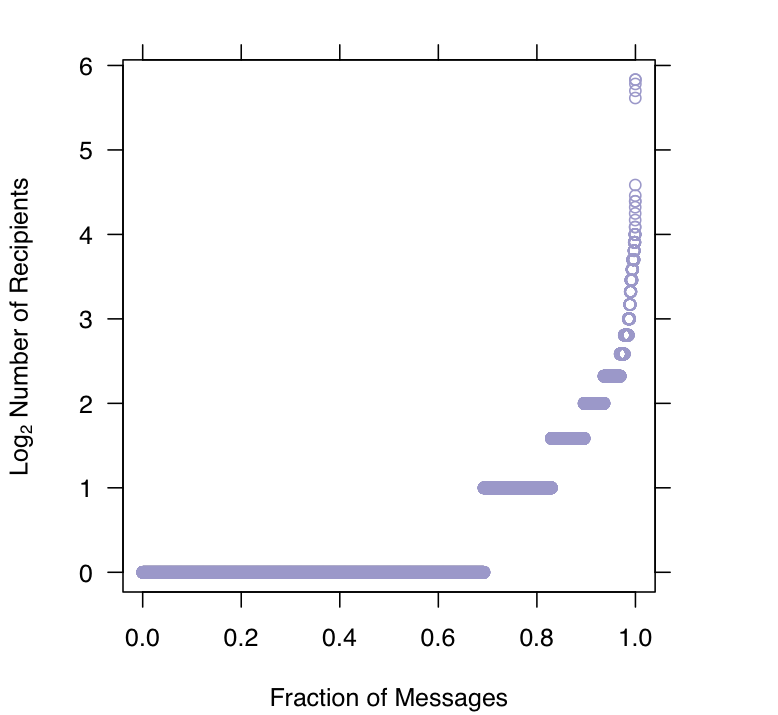
\includegraphics[scale=0.6]{figures/recipient-counts}}
    \caption{
        \captiontitle{Message recipient counts}
        Each of the 21,635 points corresponds to a message, with
        $y$-value showing the base-2 logarithm of its number of recipients
        (ranging from 1--57).
    }\label{F:recipient-counts}
\end{figure}
In the subsequent analysis, we exclude messages with more than 10
recipients---a subjectively-chosen cutoff that avoids e-mails sent
\emph{en masse} to large groups.

We model these data using the multicast proportional intensity
model of Section~\ref{S:multiple-receivers}, with
$\mathcal{I} = \mathcal{J} = \{ 1, 2, \ldots, 156 \}$ and
$\mathcal{J}_t(i) = \mathcal{I} \setminus \{ i \}$, and with static and
dynamic covariates described in the next section.
We fit the model by first maximizing the approximate log partial
likelihood $\log \widetilde{\mathit{PL}}_t(\beta)$ of~\eqref{E:log-pl-multiple-approx}, and then employing a
parametric bootstrap to estimate and correct the resultant bias in
parameter estimates.  Standard errors are calculated using the
corresponding asymptotic theory, along with the delta method as
appropriate.  Note that in the setting of this data analysis example,
the covariates are bounded and the interaction count is high, and so
assumptions A\ref{A:square-int}--A\ref{A:var-equicont} and the asymptotic
framework developed in Sections~\ref{S:MPLE-consistency}
and~\ref{S:multiple-receivers} are natural.

\subsection{Covariates}

To assess the predictiveness of an effect (trait or behavior) in the
in the proportional intensity model~\eqref{E:cox-intensity}, we must encode it in the time-varying covariate vector $x_t(i,j)$.

\subsubsection{Static covariates to measure homophily and group-level effects}

Consider first those actor traits that do not vary with time: the actors' genders, departments, and seniorities.  We encode the traits of actor $i$ and their second-order interactions using 9 actor-dependent binary ($0$/$1$) variables:

\begin{center}
\begin{tabular}{clc}
\hline
Variate & Characteristic of actor $i$ & Count \\
\hline
$L(i)$ & member of the Legal department & 25 \\
$T(i)$ & member of the Trading department & 60 \\
$J(i)$ & seniority is Junior & 82 \\
$F(i)$ & gender is Female & 43 \\
$LJ(i)$ & $L(i) \cdot J(i)$ & ??? \\
$TJ(i)$ & $T(i) \cdot J(i)$ & ??? \\
$LF(i)$ & $L(i) \cdot F(i)$ & ??? \\
$TF(i)$ & $T(i) \cdot F(i)$ & ??? \\
$JF(i)$ & $J(i) \cdot F(i)$ & ??? \\
\hline
\end{tabular}
\end{center}

We encode all 90 identifiable second-order interactions between the traits of sender $i$ and receiver $j$ as components of $x_t(i,j)$.  We do this by using variates of the form $Y(j)$ and $X(i)\cdot Y(j)$, where $X$ and $Y$ are chosen from the list of 9 actor-dependent variates ($L$, $T$, $J$, $F$, $LJ$, etc.).  We cannot identify the coefficients for covariates of the form $X(i)$; if a component of $x_t(i,j)$ is the same for all values of $j$, then the corresponding component of $\beta$ will not be identifiable; the product of the two can be absorbed into $\bar \lambda_t(i)$ without changing the likelihood.

We measure homophily be the estimated coefficients for covariates of the form $X(i) \cdot X(j)$.  For example, if the coefficient of $J(i) \cdot J(j)$ is large and positive, this tells us that Junior employees exhibit homophily in their sending behaviors.


\subsubsection{Dynamic covariates to measure network effects}

Static effects are useful for determining which traits are predictive of the relative rate of interaction between sender $i$ and receiver $j$, but they do not shed light on network effects.  We are interested in the predictive relevance of the following dynamic behaviors:

\vspace{1em}
\begin{tabular}{p{2cm} c p{8cm}}
  \textbf{send} &
    \vspace{1em}
    \setlength{\unitlength}{1em}
    \begin{picture}(4.75,1)
      \put(0,0){$i$}
      \put(1,0.25){\vector(1,0){2.5}}
      \put(4,0){$j$}
      \end{picture} &
    $i$ has sent $j$ a message in the past
    \\
  \textbf{receive} &
    \vspace{1em}
    \setlength{\unitlength}{1em}
    \begin{picture}(4.75,1)
      \put(0,0){$i$}
      \put(3.5,0.25){\vector(-1,0){2.5}}
      \put(4,0){$j$}
    \end{picture} &
    $i$ has received a message from $j$ in the past
    \\
  \textbf{$2$-send} &
    \vspace{1em}
    \setlength{\unitlength}{1em}
    \begin{picture}(9,1)
      \put(0,0){$i$}
      \put(1,0.25){\vector(1,0){2.5}}
      \put(4,0){$h$}
      \put(5,0.25){\vector(1,0){2.5}}
      \put(8.25,0){$j$}
    \end{picture} &
    there exists an actor $h$ such that $i$ has sent $h$ a message
    and $h$ has sent $j$ a message in the past
    \\
  \textbf{$2$-receive} &
    \vspace{-3em}
    \setlength{\unitlength}{1em}
    \begin{picture}(9,1)
      \put(0,0){$i$}
      \put(3.5,0.25){\vector(-1,0){2.5}}
      \put(4,0){$h$}
      \put(7.75,0.25){\vector(-1,0){2.5}}
      \put(8.25,0){$j$}
    \end{picture} &
    there exists an actor $h$ such that $i$ has received a message 
    from $h$, and $h$ has received a message from~$j$
    \\
  \textbf{sibling} &
    \setlength{\unitlength}{1em}
    \begin{picture}(5,5)(0,4)
      \put(2.5,4){$h$}
      \put(2.5,3.5){\vector(-1,-2){1.25}}
      \put(2.75,3.5){\vector(1,-2){1.25}}
      \put(1,0){$i$}
      \put(3.75,0){$j$}
    \end{picture} &
    there exists an actor $k$ such that $h$ has sent $i$ and $j$
    messages in the past
    \\
  \textbf{cosibling} &
    \vspace{4em}
    \setlength{\unitlength}{1em}
    \begin{picture}(5,5)(0,4)
      \put(2.5,4){$h$}
      \put(1.25,1){\vector(1,2){1.25}}
      \put(4,1){\vector(-1,2){1.25}}
      \put(1,0){$i$}
      \put(3.75,0){$j$}
    \end{picture} &
    there exists an actor $h$ such that $k$ has received messages
    from $i$ and~$j$
\end{tabular}

\noindent
The first two are ``dyadic,'' involving exactly two actors, and the last four are ``triadic,'' involving exactly three actors.

To measure first-order dependence on the network effects, we introduce binary indicators for all $6$ effects as components of $x_t(i,j)$.  These indicators depend on the sender $i$, the receiver, $j$, and the history of the process at the current time $t$.

To measure higher-order time dependence, we introduce further covariates.  We partition the interval $[-\infty, t)$ into $K = 7$ sub-intervals:
\[
  [-\infty, t) = 
  [t - \Delta_K, t - \Delta_{K-1}) \cup [t - \Delta_{K-1}, t - \Delta_{K-2}) \cup \dotsb \cup [t - \Delta_1, t - \Delta_0)
\]
where $\infty = \Delta_K > \Delta_{K-1} > \dotsb > \Delta_1 > \Delta_0 = 0$ and ``$t - \infty$'' is defined to be $-\infty$.  Specifically, we set $\Delta_k = (7.5\text{ minutes}) \times 4^k$ for $k = 1, \dotsc, K-1$ so that for $k$ in this range $\Delta_k$ takes the values $30\text{ minutes}$, $2\text{ hours}$, $8\text{ hours}$, $32\text{ hours}$, $5.33\text{ days}$, $21.33\text{ days}$.  We define the half-open interval $I_{t}^{(k)} = [t - \Delta_k, t - \Delta_{k-1})$.

For $k = 1, \dotsc, K$ we define the dyadic effects
\begin{align*}
  \text{\textbf{send}}^{(k)}_t(i,j)
    &= \#\{ i \to j \text{ in } I_t^{(k)} \}, \\
  \text{\textbf{receive}}^{(k)}_t(i,j)
    &= \#\{ j \to i \text{ in } I_t^{(k)} \};
\end{align*}
for sender $i$, these covariates measure the number of messages sent-to and received-by receiver $j$ in time interval $I_t^{(k)}$.  

The dyadic effects have been defined as above to enable easy interpretation of the corresponding coefficients.  To illustrate this, for $k = 1, \dotsc, K$, suppose that $\beta_{k}$ is the coeffiecient corresponding to $\text{\textbf{send}}^{(k)}_t(i,j)$.  If we observe the message $i \to j$ at time $t$, then for future time $t'$ in the interval $(t, t + \Delta_1]$, the rate $\lambda_{t'}(i,j)$ will be multiplied be the factor $e^{\beta_{1}}$; for $t'$ in the interval $(t + \Delta_1, t + \Delta_2]$, the rate will be multiplied by $e^{\beta_{2}}$; this continues similarly, with the rate being multiplied by $e^{\beta_{k}}$ whenever $t' \in (t + \Delta_{k-1}, t + \Delta_{k}]$; equivalently, when $\Delta_{k-1} < t' - t \leq \Delta_k$.  Thus, the coefficients $\beta_{1}, \dotsc, \beta_{K}$ measure the effect of a ``send event'' and how this effect decays over time. 
We expect that $\beta_{k}$ will decrease as $k$ increases, but we do not enforce this constraint on the estimation procedure.  

The triadic effects involve pairs of messages.  For $k = 1, \dotsc, K$ and $l = 1, \dotsc, K$ we define the triadic effects
\begin{align*}
  \text{\textbf{2-send}}^{(k,l)}_t(i,j)
    &= \sum_{h \neq i,j} 
      \#\{ i \to h \text{ in } I_t^{(k)} \}
      \cdot \#\{ h \to j \text{ in } I_t^{(l)} \}, \\
  \text{\textbf{2-receive}}^{(k,l)}_t(i,j)
    &= \sum_{h \neq i,j} 
      \#\{ h \to i \text{ in } I_t^{(k)} \}
      \cdot \#\{ j \to h \text{ in } I_t^{(l)} \}, \\
  \text{\textbf{sibling}}^{(k,l)}_t(i,j)
    &= \sum_{h \neq i,j} 
      \#\{ h \to i \text{ in } I_t^{(k)} \}
      \cdot \#\{ h \to j \text{ in } I_t^{(l)} \}, \\
  \text{\textbf{cosibling}}^{(k,l)}_t(i,j)
    &= \sum_{h \neq i,j} 
      \#\{ i \to h \text{ in } I_t^{(k)} \}
      \cdot \#\{ j \to h \text{ in } I_t^{(l)} \}.
\end{align*}
For sender $i$ and receiver $j$, the covariate
$\text{\textbf{2-send}}^{(k,l)}_t(i,j)$ counts the pairs of messages such that for some $h$ distinct from $i$ and $j$, message $i \to h$ occurred in interval $I_t^{(k)}$ and message $h \to j$ occurred in interval $I_t^{(l)}$; the other covariates behave similarly.

As with the dyadic effects, the triadic effects are designed so that their coefficients have a straightforward interpretation.  However, since triadic effects involve pairs of messages, the interpretation is a bit more involved.  We illustrate with the $\text{\textbf{2-send}}^{(k,l)}_t(i,j)$ covariate having coefficient $\beta_{k,l}$ for $k = 1, \dotsc, K$ and $l = 1, \dotsc, K$.  Take $i$ and $j$ to be two actors.  Suppose at time $t$ we observe the message $h \to j$.  At this point, we look through the history of the process for all messages of the form $i \to h$; when paired with the original $h \to j$ message, each of these defines a ``2-send event.''  The other 2-send events are defined as follows: if at time $s$ we observe the message $i \to h$, then we enumerate all observed messages $h \to j$ in the history of the process; when each of these is paired with the original $i \to h$ event it constitutes a 2-send event.  A pair $(s,t)$ can be associated with each 2-send event, where $s$ is the time of the $i \to h$ message and $t$ is the time of the $h \to j$ message.  At time $t'$ after $s$ and $t$, the existence of the 2-send event causes the sending rate $\lambda_{t'}(i,j)$ to be multiplied by the factor $e^{\beta_{k,l}}$, where $\Delta_{k-1} < t' - s \leq \Delta_{k}$ and $\Delta_{l-1} < t' - t \leq \Delta_l$.  We expect $\beta_{k,l}$ to decrease as $k$, $l$, and $|k - l|$ increase (again, we do not enforce this constraint in the fitting procedure).


\subsection{Estimation}

\subsection{Goodness of fit}

\subsection{Analysis 1: Testing for homophily}

%%% Logically, this should be a 'table', not a 'figure', but I can't get it
%%% to work with the JRSS 'statsoc.cls' file (I spent 2 hours on this and
%%% then gave up).
\begin{figure}
  \centering
  \subfloat[Static]{
    \label{T:group:static}
    \scriptsize
    \makebox[\textwidth]{\begin{tabular}{lrrrrrrrrrr}
\toprule
& \multicolumn{10}{c}{Receiver} \\
\cmidrule(l){2-11} 
Sender & \multicolumn{1}{c}{1} & \multicolumn{1}{c}{L} & \multicolumn{1}{c}{T} & \multicolumn{1}{c}{J} & \multicolumn{1}{c}{F} & \multicolumn{1}{c}{LJ} & \multicolumn{1}{c}{TJ} & \multicolumn{1}{c}{LF} & \multicolumn{1}{c}{TF} & \multicolumn{1}{c}{JF} \\
\midrule
\multirow{2}{*}{L} &-0.22 &\cellcolor{Gray}1.96 &\textcolor{LightGray}{-0.03} &-1.87 &-0.67 &0.85 &2.64 &2.02 &\textcolor{LightGray}{1.08} &0.82\\
 &\tiny{(0.05)} &\cellcolor{Gray}\tiny{(0.06)} &\textcolor{LightGray}{\tiny{(0.11)}} &\tiny{(0.22)} &\tiny{(0.09)} &\tiny{(0.21)} &\tiny{(0.30)} &\tiny{(0.13)} &\textcolor{LightGray}{\tiny{(0.41)}} &\tiny{(0.15)}\\[1ex]
\multirow{2}{*}{T} &-1.95 &-0.59 &\cellcolor{Gray}2.58 &2.76 &-0.45 &\textcolor{LightGray}{0.20} &-1.72 &1.05 &3.19 &-1.65\\
 &\tiny{(0.06)} &\tiny{(0.09)} &\cellcolor{Gray}\tiny{(0.08)} &\tiny{(0.10)} &\tiny{(0.10)} &\textcolor{LightGray}{\tiny{(0.15)}} &\tiny{(0.18)} &\tiny{(0.16)} &\tiny{(0.32)} &\tiny{(0.13)}\\[1ex]
\multirow{2}{*}{J} &-3.21 &-2.49 &2.56 &\cellcolor{Gray}4.26 &\textcolor{LightGray}{0.19} &-1.47 &-1.70 &1.95 &2.26 &-1.65\\
 &\tiny{(0.09)} &\tiny{(0.19)} &\tiny{(0.11)} &\cellcolor{Gray}\tiny{(0.12)} &\textcolor{LightGray}{\tiny{(0.12)}} &\tiny{(0.24)} &\tiny{(0.19)} &\tiny{(0.23)} &\tiny{(0.32)} &\tiny{(0.15)}\\[1ex]
\multirow{2}{*}{F} &\textcolor{LightGray}{-0.09} &-0.62 &\textcolor{LightGray}{-0.16} &\textcolor{LightGray}{0.14} &\cellcolor{Gray}0.71 &0.86 &-3.85 &\textcolor{LightGray}{-0.14} &\textcolor{LightGray}{0.83} &\textcolor{LightGray}{-0.36}\\
 &\textcolor{LightGray}{\tiny{(0.05)}} &\tiny{(0.08)} &\textcolor{LightGray}{\tiny{(0.10)}} &\textcolor{LightGray}{\tiny{(0.12)}} &\cellcolor{Gray}\tiny{(0.07)} &\tiny{(0.17)} &\tiny{(0.28)} &\textcolor{LightGray}{\tiny{(0.17)}} &\textcolor{LightGray}{\tiny{(0.31)}} &\textcolor{LightGray}{\tiny{(0.14)}}\\[1ex]
\multirow{2}{*}{LJ} &1.53 &1.18 &\textcolor{LightGray}{0.01} &-1.35 &\textcolor{LightGray}{0.15} &\cellcolor{Gray}\textcolor{LightGray}{0.76} &-3.03 &-1.68 &\textcolor{LightGray}{0.56} &0.98\\
 &\tiny{(0.16)} &\tiny{(0.22)} &\textcolor{LightGray}{\tiny{(0.21)}} &\tiny{(0.32)} &\textcolor{LightGray}{\tiny{(0.23)}} &\cellcolor{Gray}\textcolor{LightGray}{\tiny{(0.36)}} &\tiny{(0.41)} &\tiny{(0.30)} &\textcolor{LightGray}{\tiny{(0.49)}} &\tiny{(0.21)}\\[1ex]
\multirow{2}{*}{TJ} &1.43 &4.29 &-1.65 &-2.00 &-1.53 &-2.15 &\cellcolor{Gray}\textcolor{LightGray}{0.40} &\textcolor{LightGray}{0.68} &\textcolor{LightGray}{-1.21} &1.15\\
 &\tiny{(0.18)} &\tiny{(0.26)} &\tiny{(0.20)} &\tiny{(0.20)} &\tiny{(0.24)} &\tiny{(0.32)} &\cellcolor{Gray}\textcolor{LightGray}{\tiny{(0.26)}} &\textcolor{LightGray}{\tiny{(0.32)}} &\textcolor{LightGray}{\tiny{(0.37)}} &\tiny{(0.22)}\\[1ex]
\multirow{2}{*}{LF} &-2.82 &2.13 &\textcolor{LightGray}{0.50} &\textcolor{LightGray}{0.66} &\textcolor{LightGray}{0.70} &\textcolor{LightGray}{-0.55} &5.29 &\cellcolor{Gray}\textcolor{LightGray}{-0.04} &-2.48 &\textcolor{LightGray}{-0.59}\\
 &\tiny{(0.18)} &\tiny{(0.19)} &\textcolor{LightGray}{\tiny{(0.25)}} &\textcolor{LightGray}{\tiny{(0.34)}} &\textcolor{LightGray}{\tiny{(0.25)}} &\textcolor{LightGray}{\tiny{(0.35)}} &\tiny{(0.45)} &\cellcolor{Gray}\textcolor{LightGray}{\tiny{(0.29)}} &\tiny{(0.40)} &\textcolor{LightGray}{\tiny{(0.20)}}\\[1ex]
\multirow{2}{*}{TF} &-2.57 &\textcolor{LightGray}{-0.09} &2.83 &2.15 &0.99 &\textcolor{LightGray}{-0.17} &1.40 &\textcolor{LightGray}{-0.94} &\cellcolor{Gray}-2.41 &\textcolor{LightGray}{-0.25}\\
 &\tiny{(0.28)} &\textcolor{LightGray}{\tiny{(0.36)}} &\tiny{(0.29)} &\tiny{(0.29)} &\tiny{(0.27)} &\textcolor{LightGray}{\tiny{(0.39)}} &\tiny{(0.36)} &\textcolor{LightGray}{\tiny{(0.29)}} &\cellcolor{Gray}\tiny{(0.33)} &\textcolor{LightGray}{\tiny{(0.26)}}\\[1ex]
\multirow{2}{*}{JF} &1.88 &0.91 &-1.38 &-1.46 &-0.53 &\textcolor{LightGray}{0.30} &2.09 &\textcolor{LightGray}{-0.04} &\textcolor{LightGray}{0.13} &\cellcolor{Gray}\textcolor{LightGray}{0.54}\\
 &\tiny{(0.11)} &\tiny{(0.15)} &\tiny{(0.14)} &\tiny{(0.15)} &\tiny{(0.14)} &\textcolor{LightGray}{\tiny{(0.20)}} &\tiny{(0.21)} &\textcolor{LightGray}{\tiny{(0.19)}} &\textcolor{LightGray}{\tiny{(0.29)}} &\cellcolor{Gray}\textcolor{LightGray}{\tiny{(0.17)}}\\[1ex]
\bottomrule
\end{tabular}
}
  }
  \\
  \subfloat[Static and dynamic]{
    \label{T:group:dynamic}
    \scriptsize
    \makebox[\textwidth]{\begin{tabular}{lrrrrrrrrrr}
\toprule
& \multicolumn{10}{c}{Receiver} \\
\cmidrule(l){2-11} 
Sender & \multicolumn{1}{c}{1} & \multicolumn{1}{c}{L} & \multicolumn{1}{c}{T} & \multicolumn{1}{c}{J} & \multicolumn{1}{c}{F} & \multicolumn{1}{c}{LJ} & \multicolumn{1}{c}{TJ} & \multicolumn{1}{c}{LF} & \multicolumn{1}{c}{TF} & \multicolumn{1}{c}{JF} \\
\midrule
\multirow{2}{*}{L} &-0.50 &\cellcolor{Gray}0.19 &0.19 &-0.41 &-0.03 &0.43 &0.39 &1.05 &1.05 &\textcolor{LightGray}{-0.02}\\
 &\tiny{(0.00)} &\cellcolor{Gray}\tiny{(0.00)} &\tiny{(0.04)} &\tiny{(0.03)} &\tiny{(0.00)} &\tiny{(0.03)} &\tiny{(0.05)} &\tiny{(0.02)} &\tiny{(0.04)} &\textcolor{LightGray}{\tiny{(0.04)}}\\[1ex]
\multirow{2}{*}{T} &-0.35 &-0.23 &\cellcolor{Gray}0.72 &0.66 &-0.02 &0.38 &-0.46 &0.40 &0.99 &-0.52\\
 &\tiny{(0.00)} &\tiny{(0.00)} &\cellcolor{Gray}\tiny{(0.04)} &\tiny{(0.02)} &\tiny{(0.00)} &\tiny{(0.05)} &\tiny{(0.05)} &\tiny{(0.01)} &\tiny{(0.04)} &\tiny{(0.02)}\\[1ex]
\multirow{2}{*}{J} &-0.40 &-1.23 &0.64 &\cellcolor{Gray}0.57 &-0.21 &\textcolor{LightGray}{0.12} &\textcolor{LightGray}{-0.03} &1.31 &0.62 &\textcolor{LightGray}{-0.02}\\
 &\tiny{(0.00)} &\tiny{(0.01)} &\tiny{(0.03)} &\cellcolor{Gray}\tiny{(0.01)} &\tiny{(0.00)} &\textcolor{LightGray}{\tiny{(0.04)}} &\textcolor{LightGray}{\tiny{(0.03)}} &\tiny{(0.01)} &\tiny{(0.03)} &\textcolor{LightGray}{\tiny{(0.01)}}\\[1ex]
\multirow{2}{*}{F} &-0.08 &\textcolor{LightGray}{0.13} &0.22 &0.09 &\cellcolor{Gray}0.38 &\textcolor{LightGray}{-0.00} &-1.40 &\textcolor{LightGray}{-0.25} &0.20 &-0.14\\
 &\tiny{(0.00)} &\textcolor{LightGray}{\tiny{(0.08)}} &\tiny{(0.03)} &\tiny{(0.01)} &\cellcolor{Gray}\tiny{(0.00)} &\textcolor{LightGray}{\tiny{(0.08)}} &\tiny{(0.03)} &\textcolor{LightGray}{\tiny{(0.08)}} &\tiny{(0.03)} &\tiny{(0.01)}\\[1ex]
\multirow{2}{*}{LJ} &0.99 &0.73 &-0.67 &-0.33 &-0.82 &\cellcolor{Gray}-0.67 &-1.48 &-0.31 &1.20 &0.41\\
 &\tiny{(0.00)} &\tiny{(0.04)} &\tiny{(0.01)} &\tiny{(0.00)} &\tiny{(0.00)} &\cellcolor{Gray}\tiny{(0.05)} &\tiny{(0.01)} &\tiny{(0.04)} &\tiny{(0.01)} &\tiny{(0.05)}\\[1ex]
\multirow{2}{*}{TJ} &0.07 &1.79 &-0.51 &-0.27 &-0.95 &-1.25 &\cellcolor{Gray}\textcolor{LightGray}{0.01} &\textcolor{LightGray}{0.11} &0.22 &0.34\\
 &\tiny{(0.00)} &\tiny{(0.03)} &\tiny{(0.00)} &\tiny{(0.00)} &\tiny{(0.00)} &\tiny{(0.03)} &\cellcolor{Gray}\textcolor{LightGray}{\tiny{(0.00)}} &\textcolor{LightGray}{\tiny{(0.05)}} &\tiny{(0.00)} &\tiny{(0.03)}\\[1ex]
\multirow{2}{*}{LF} &-1.12 &1.35 &0.63 &-0.21 &0.34 &0.28 &2.83 &\cellcolor{Gray}-0.55 &-1.77 &-0.22\\
 &\tiny{(0.02)} &\tiny{(0.03)} &\tiny{(0.02)} &\tiny{(0.02)} &\tiny{(0.02)} &\tiny{(0.03)} &\tiny{(0.02)} &\cellcolor{Gray}\tiny{(0.03)} &\tiny{(0.02)} &\tiny{(0.03)}\\[1ex]
\multirow{2}{*}{TF} &-0.72 &0.36 &0.99 &0.58 &0.43 &-0.15 &0.61 &-0.27 &\cellcolor{Gray}-1.05 &-0.25\\
 &\tiny{(0.02)} &\tiny{(0.02)} &\tiny{(0.02)} &\tiny{(0.02)} &\tiny{(0.02)} &\tiny{(0.02)} &\tiny{(0.02)} &\tiny{(0.02)} &\cellcolor{Gray}\tiny{(0.02)} &\tiny{(0.03)}\\[1ex]
\multirow{2}{*}{JF} &\textcolor{LightGray}{0.02} &-0.10 &\textcolor{LightGray}{-0.20} &\textcolor{LightGray}{0.01} &0.14 &0.40 &\textcolor{LightGray}{-0.18} &-0.67 &\textcolor{LightGray}{-0.09} &\cellcolor{Gray}0.17\\
 &\textcolor{LightGray}{\tiny{(0.01)}} &\tiny{(0.01)} &\textcolor{LightGray}{\tiny{(0.07)}} &\textcolor{LightGray}{\tiny{(0.02)}} &\tiny{(0.01)} &\tiny{(0.04)} &\textcolor{LightGray}{\tiny{(0.07)}} &\tiny{(0.01)} &\textcolor{LightGray}{\tiny{(0.07)}} &\cellcolor{Gray}\tiny{(0.02)}\\[1ex]
\bottomrule
\end{tabular}
}
  }
  \caption{Group effects}
  \label{T:group}
\end{figure}

\FloatBarrier

Darker coefficients are significant (according to a Wald test) at level $10^{-3}$.

\subsection{Analysis 2: Evaluating the importance of network effects}

\begin{figure}
  \centering
  \makebox{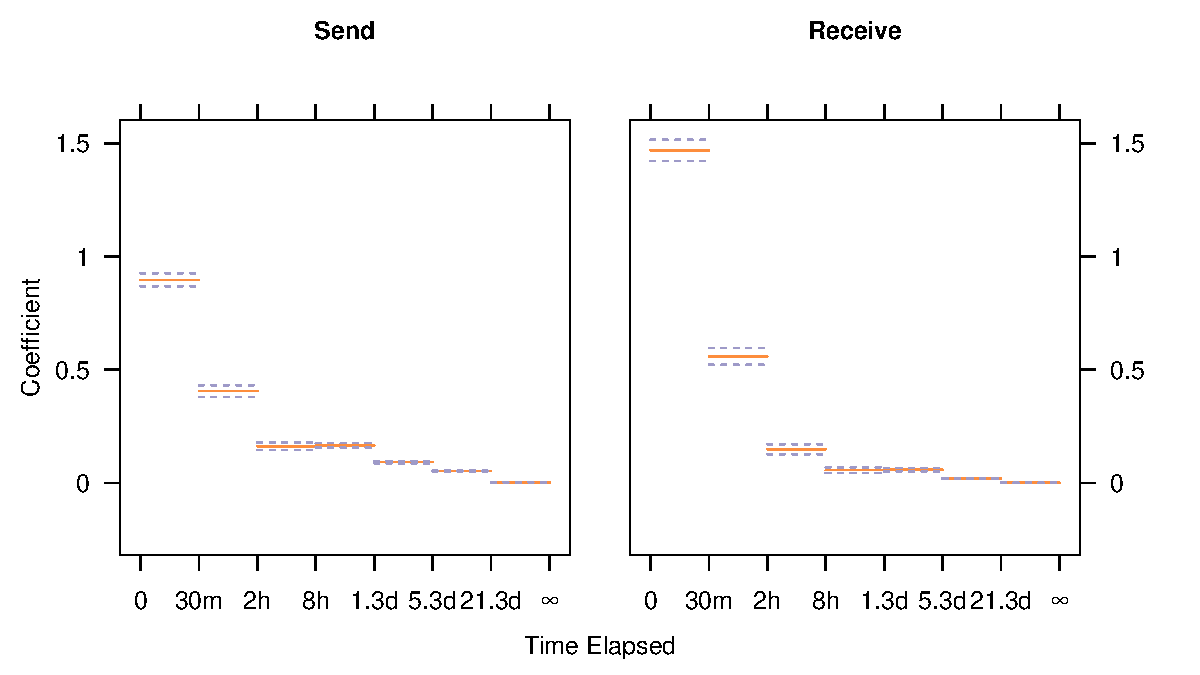
\includegraphics[scale=0.6]{figures/dyad}}
  \caption{Estimated coefficients for dyadic effects}
\end{figure}



\clearpage
The $21$ dynamic
components of $x_t(i,j)$ are history-dependent and designed to capture
reciprocation effects; they take the form
\[
    1\{\text{$j$'s most recent message to $i$ was sent in
             $[t-2^k \text{ hours}, t)$\}},
\]
where $k$ ranges from $-6$ to $14$, yielding time intervals from
$56.25$ seconds to $1.87$ years.  (Effects involving intervals outside
of this range were initially included in the model but were not found
to be significant.)

Note that the components of $\beta_0$ corresponding to the static
covariates are not identifiable, since any $\tilde \beta_0$ satisfying
$\tilde \beta_0^\trans x_t(i,j) = \beta_0^\trans x_t(i,j) + \alpha_t(i)$
gives rise to the same partial likelihood.  We identify $\beta_0$ by by
imposing sum-to-zero constraints within each of the $12$ receiver
classes, reducing the corresponding degrees of freedom from $144$ to $132$.

\subsection{Results}

Given the model specification, data, and covariates outlined above, we can
estimate the parameter vector $\beta_0$ under the approximate
log partial likelihood of~\eqref{E:log-pl-multiple-approx}.  Recall
that the results of Section~\ref{S:multiple-receivers} bound the bias
resulting from this approximate MPLE procedure as a function of the growth
rate of the recipient set $\mathcal{J}$ over time.  Here, treating the
set $\mathcal{J}$ of 156 Enron employees as constant, the resultant bias
is of order $1/|\mathcal{J}|$---and, since $|\mathcal{J}| = 156$ is on the
order of the square root of the number 21,365 of messages in the dataset,
we can correct this bias using the parametric bootstrap outlined at the
end of Section~\ref{S:multiple-receivers}.  Fig.~\ref{F:boot-resid}
\begin{figure}[t]
    \centering
    \makebox{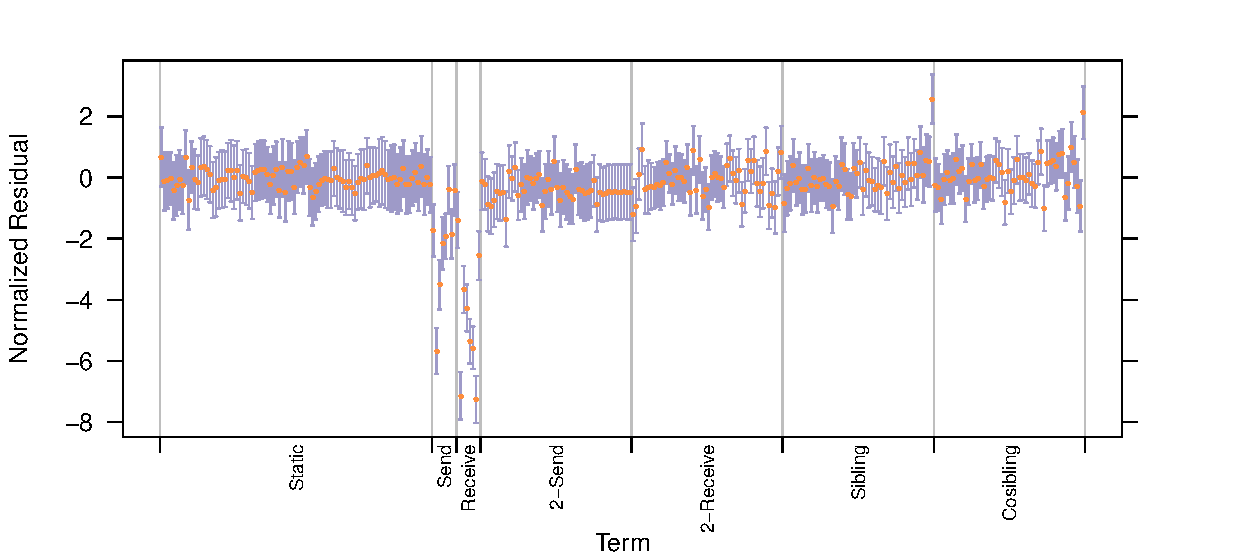
\includegraphics[scale=0.6]{figures/boot-resid}}
    \caption{
        \captiontitle{Enron bootstrap residuals}
        Summary of bootstrap residuals
        for estimated coefficients using the Enron dataset, normalized by
        estimated standard errors.  The points (orange) show the means, and
        the error bars (purple) show one standard deviation.  Coefficients
        1--144 are the group-level (static) effects, and coefficients
        145--165 are the reciprocation (dynamic) effects, ordered from
        shortest time interval to longest.  The bias is on the order of
        the standard error, and is near zero for most---but not all---of the
        coefficients.
    }
    \label{F:boot-resid}
\end{figure}
summarizes the corresponding bootstrap residuals (from $500$ replicates) for
each component of the estimated parameter vector $\beta_0$; we can see from
this figure that treating messages with multiple recipients as multiple
single-recipient messages leads to negative bias in the coefficient
estimates.

\newcommand{\refTgroupeffects}{2} % \ref{T:group-effects}
The bias-corrected results of inference on $\beta_0$ are summarized as
follows.  Table~\refTgroupeffects
%\begin{table}
%    \tiny
%    \makebox[\textwidth]{
\begin{tabular}{ll@{\,\,\,}rl@{\,\,\,}rl@{\,\,\,}rl@{\,\,\,}rl@{\,\,\,}rl@{\,\,\,}r}
\toprule
    & \multicolumn{12}{c}{\textbf{Sender}} \\
    \cmidrule(lr){2- 13 }
\textbf{Receiver}
    & \multicolumn{2}{c}{\textnormal{FLJ}}
    & \multicolumn{2}{c}{\textnormal{FLS}}
    & \multicolumn{2}{c}{\textnormal{FTJ}}
    & \multicolumn{2}{c}{\textnormal{FTS}}
    & \multicolumn{2}{c}{\textnormal{FOJ}}
    & \multicolumn{2}{c}{\textnormal{FOS}} \\
    \cmidrule(lr){1-1}
    \cmidrule(lr){2-3}
    \cmidrule(lr){4-5}
    \cmidrule(lr){6-7}
    \cmidrule(lr){8-9}
    \cmidrule(lr){10-11}
    \cmidrule(lr){12-13}
    \textnormal{FLJ} & \textbf{3.31} & (0.11) & 3.06 & (0.25) & 1.55 & (0.30) & 1.25 & (0.35) & 0.29 & (0.08) & 0.69 & (0.10) \\
    \textnormal{FLS} & 2.55 & (0.11) & 4.21 & (0.41) & 0.15 & (0.14) & 0.76 & (0.37) & 0.39 & (0.15) & 1.00 & (0.20) \\
    \textnormal{FTJ} & 0.43 & (0.06) & 0.61 & (0.24) & 1.36 & (0.33) & 1.39 & (0.38) & 0.46 & (0.12) & 1.00 & (0.29) \\
    \textnormal{FTS} & 0.81 & (0.12) & 0.49 & (0.14) & \textbf{4.34} & (1.11) & \textbf{2.53} & (0.65) & 2.22 & (0.28) & 0.19 & (0.10) \\
    \textnormal{FOJ} & 0.47 & (0.05) & 0.14 & (0.06) & 0.96 & (0.29) & 1.54 & (0.27) & \textbf{2.86} & (0.23) & 1.92 & (0.18) \\
    \textnormal{FOS} & 0.99 & (0.07) & 1.11 & (0.19) & 0.11 & (0.09) & 0.70 & (0.34) & 1.46 & (0.16) & \textbf{3.84} & (0.30) \\
    \textnormal{MLJ} & 1.41 & (0.10) & 1.03 & (0.28) & 3.62 & (0.69) & 0.65 & (0.42) & 1.48 & (0.32) & 0.76 & (0.15) \\
    \textnormal{MLS} & 3.07 & (0.11) & \textbf{4.48} & (0.35) & 1.15 & (0.45) & 0.65 & (0.21) & 0.35 & (0.09) & 1.48 & (0.14) \\
    \textnormal{MTJ} & 0.70 & (0.06) & 1.42 & (0.18) & 2.10 & (0.38) & 0.61 & (0.17) & 0.66 & (0.10) & 0.33 & (0.08) \\
    \textnormal{MTS} & 0.61 & (0.05) & 1.32 & (0.15) & 2.68 & (0.41) & 2.16 & (0.29) & 1.58 & (0.14) & 0.99 & (0.10) \\
    \textnormal{MOJ} & 0.47 & (0.04) & 0.27 & (0.05) & 2.16 & (0.35) & 1.34 & (0.21) & 1.62 & (0.13) & 0.75 & (0.08) \\
    \textnormal{MOS} & 0.86 & (0.06) & 0.71 & (0.10) & 0.13 & (0.10) & 0.37 & (0.14) & 2.39 & (0.20) & 3.74 & (0.28) \\
\end{tabular}

\begin{tabular}{ll@{\,\,\,}rl@{\,\,\,}rl@{\,\,\,}rl@{\,\,\,}rl@{\,\,\,}rl@{\,\,\,}r}
\phantom{\textbf{Receiver}} &\\
    & \multicolumn{2}{c}{\textnormal{MLJ}}
    & \multicolumn{2}{c}{\textnormal{MLS}}
    & \multicolumn{2}{c}{\textnormal{MTJ}}
    & \multicolumn{2}{c}{\textnormal{MTS}}
    & \multicolumn{2}{c}{\textnormal{MOJ}}
    & \multicolumn{2}{c}{\textnormal{MOS}} \\
    \cmidrule(lr){2-3}
    \cmidrule(lr){4-5}
    \cmidrule(lr){6-7}
    \cmidrule(lr){8-9}
    \cmidrule(lr){10-11}
    \cmidrule(lr){12-13}
    \textnormal{FLJ} & 2.21 & (0.24) & 2.97 & (0.24) & 0.27 & (0.07) & 0.08 & (0.02) & 0.14 & (0.06) & 0.70 & (0.12) \\
    \textnormal{FLS} & 0.45 & (0.24) & 2.46 & (0.21) & 2.33 & (0.35) & 0.42 & (0.08) & 0.11 & (0.07) & 0.38 & (0.09) \\
    \textnormal{FTJ} & 2.14 & (0.32) & 0.06 & (0.05) & \textbf{6.19} & (0.56) & \textbf{2.26} & (0.17) & 3.13 & (0.35) & 0.06 & (0.05) \\
    \textnormal{FTS} & 0.44 & (0.21) & 0.48 & (0.10) & 1.18 & (0.24) & 2.00 & (0.17) & 0.51 & (0.10) & 0.39 & (0.15) \\
    \textnormal{FOJ} & 0.39 & (0.10) & 0.26 & (0.06) & 0.27 & (0.07) & 1.01 & (0.09) & 2.07 & (0.19) & 3.32 & (0.35) \\
    \textnormal{FOS} & 1.80 & (0.30) & 2.35 & (0.21) & 0.13 & (0.06) & 1.68 & (0.14) & 2.13 & (0.26) & 2.24 & (0.22) \\
    \textnormal{MLJ} & 0.94 & (0.26) & 1.52 & (0.22) & 0.70 & (0.20) & 2.24 & (0.20) & 1.04 & (0.28) & 2.26 & (0.41) \\
    \textnormal{MLS} & 1.79 & (0.22) & \textbf{6.69} & (0.51) & 0.51 & (0.12) & 0.76 & (0.07) & 0.31 & (0.09) & 2.13 & (0.21) \\
    \textnormal{MTJ} & 0.67 & (0.14) & 1.33 & (0.14) & 2.33 & (0.21) & 1.00 & (0.07) & 2.64 & (0.25) & 0.58 & (0.10) \\
    \textnormal{MTS} & \textbf{2.80} & (0.28) & 0.63 & (0.06) & 2.93 & (0.23) & 2.18 & (0.10) & 2.61 & (0.24) & 2.26 & (0.22) \\
    \textnormal{MOJ} & 0.69 & (0.14) & 0.15 & (0.03) & 3.60 & (0.28) & 1.19 & (0.07) & \textbf{4.26} & (0.36) & 0.92 & (0.11) \\
    \textnormal{MOS} & 0.69 & (0.12) & 5.75 & (0.45) & 0.71 & (0.10) & 0.84 & (0.06) & 0.96 & (0.12) & \textbf{3.53} & (0.33) \\
\bottomrule
\end{tabular}}
%    \\
%    \\
%    \caption{
%        Estimated group level effects and their standard errors for the
%        model described in Section~\ref{S:enron-modeling}.  Gender,
%        Department, and Seniority codes are abbreviated as F/M, L/T/O,
%        and J/S.  Standard errors are shown in parentheses.  Read
%        the table as follows: the group-level effect of 2.46 for sender
%        FLJ and receiver FLS means that an FLJ executive sends e-mails to a
%        FLS executive at 2.46 times her baseline activity rate.  The highest
%        effect in each column is shown in boldface.
%    }
%    \label{T:group-effects}
%\end{table}
shows the estimated group-level (static) effects, and
Fig.~\ref{F:reciprocation}
\begin{figure}[t]
    \centering
    \makebox{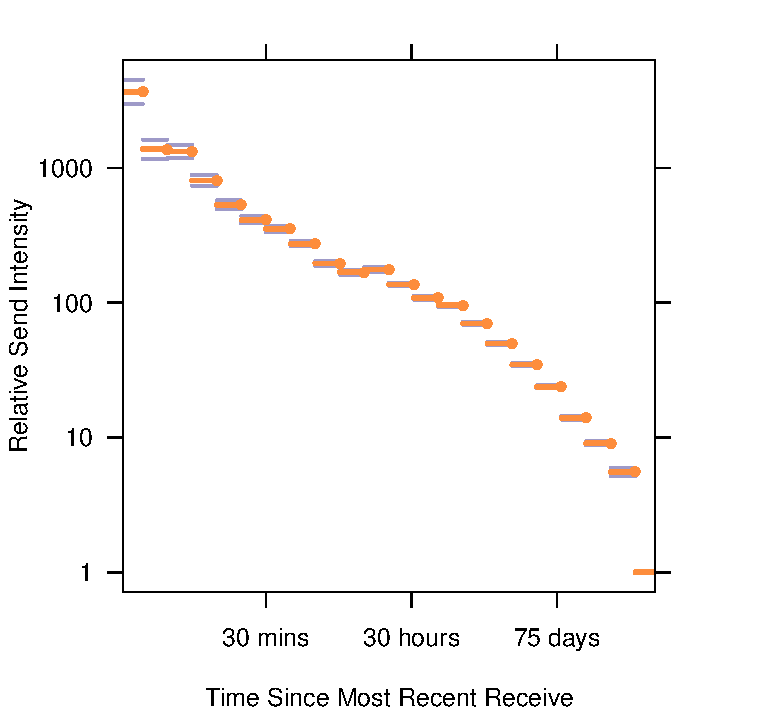
\includegraphics[scale=0.6]{figures/reciprocation-bc}}
    \caption{
        \captiontitle{Reciprocation effect}
        Estimated reciprocation effect and standard errors for the
        model described in Section~\ref{S:enron-modeling}.  The solid
        (orange) curve is determined from the 21 estimated coefficients
        for the reciprocation effects at intervals of ``\,$2^l$ hours''
        for $l$ ranging from $-6$ to $14$.  The dashed (purple) curve gives
        one standard error around the estimate.  Read the figure as follows:
        if employee $j$'s most recent message to employee $i$ was 30 minutes
        ago, then $i$ sends to $j$ at about 200 times his baseline rate.
    }\label{F:reciprocation}
\end{figure}
shows the reciprocation (dynamic) effects.  We observe that reciprocation
is stronger by orders of magnitude, amplifying the sending rate by between
about $10^1$ and $10^3$.  In contrast, group level effects are on the order
of $10^{-1}$ to $10^0$.

\newcommand{\refTdeviance}{3}%\ref{T:deviance}
Finally, Table~\refTdeviance
%\begin{table}
%    \makebox[\textwidth]{
\begin{tabular}{lrrrr}
    \toprule
    \textbf{Term}
        & \textbf{Df}
        & \textbf{Deviance}
        & \textbf{Resid. Df}
        & \textbf{Resid. Dev} \\
    \midrule
    Null &  &  & 35567 & 358759 \\
    Static & 132 & 63809 & 35435 & 294950 \\
    Dynamic & 21 & 86831 & 35414 & 208119 \\
    \bottomrule
\end{tabular}
}
%    \\
%    \\
%    \caption{
%        Ad-hoc analysis of deviance for the Enron model.  Residual deviance
%        is defined as twice the approximate negative log partial likelihood
%        from~\eqref{E:log-pl-multiple-approx}.
%        The ``Static'' term contains the group level effects, and the
%        ``Dynamic'' term contains the reciprocation effects.
%    }
%    \label{T:deviance}
%\end{table}
gives an ad-hoc analysis of deviance for the fitted model, showing that
group-level (static) effects account for 18\% of the residual deviance and
reciprocation (dynamic) effects account for 24\%.  If the model fit
perfectly, we would expect the residual deviance to be about equal to the
residual degrees of freedom; here, the residual deviance is about $5.9$
times what we would expect.  Scaling the reported standard errors by
$\sqrt{5.9}$ is an ad-hoc adjustment for this overdispersion.


\section{Discussion}\label{S:discussion}

With the increasing popularity of network science, there is an unfortunate
tendency to preprocess data into binary ties between entities.
The observables in many modeling scenarios are repeated directed interactions,
not binary ties.  Thresholding the interaction counts to obtain binary ties
gives dramatically different networks and subsequent conclusions, depending on
the choice of cutoff \citep{dechoudhury2010}.  We have avoided such arbitrary
outcomes by working directly with the observed data.

We are not the first to move beyond static tie-based representations of
network data.  There are at least two recent treatments involving point processes,
neither of which includes reciprocation effects or other covariate
information: \citet{malmgen2009characterizing} model activity at the level of
the individual using a hidden Markov model, while \citet{heard2010bayesian} work
at the level of the dyad, assuming a piecewise-constant interaction rate.
Others have considered dynamic tie-based models: see the
agent based models from social network as surveyed by
\citet{snijders2010introduction}, along with
\citefullauthor{hanneke2010discrete}'s \citeyearpar{hanneke2010discrete}
exponential random graph model with time-varying coefficients and
\citefullauthor{kolar2010estimating}'s \citeyearpar{kolar2010estimating}
time-varying stochastic block model.  Dynamic tie-based models are able
to capture some forms of reciprocation, but they are not universally
applicable since they model ties persisting in time (e.g., friendship)
instead of instantaneous events.
Aside from \citefullauthor{lunagomez2009geometric}'s \citeyearpar{lunagomez2009geometric} recent
work in the context of graphical models, interactions involving more than two
entities have largely been ignored.

The foundation of our work is Cox's \citeyearpar{cox1972regression}
proportional intensity model and
partial likelihood theory, tools which he first introduced almost
forty years ago and which have been significantly developed since
then \citep{cox1975partial, fleming1991counting, andersen1993statistical, martinussen2006dynamic, cook2007statistical}.
These tools are used extensively in the context of survival analysis, but
require further development for use in modeling interaction data.
In this vein, we have extended the associated theory in
two directions: first, we have provided results that are asymptotic in time
rather than in the size of the population under study; and second, we
have shown that treating multicast interactions via duplication leads to
bias in the parameter estimates (which can in turn be corrected in
certain regimes).  As far as we are aware, this is the first time
such a model has been brought directly to bear on relational data in
the form of a network of directed interactions.

Our analysis of the Enron corpus has demonstrated that static and
dynamic effects are both evident in e-mail communication, and we expect this
to hold broadly for other types of interactions.  The proportional intensity
model with time-varying covariates is a simple, flexible, and
well-established model for incorporating these effects into the analysis
of interaction data.


\section*{Acknowledgement}

The authors thank Joe Blitzstein, Susan Holmes, Art Owen, and Andrew Thomas
for helpful remarks and encouragement.
Work supported in part by the Army Research Office under
PECASE Award W911NF-09-1-0555 and by the Office of Naval
Research under MURI Award 58153-MA-MUR.


\appendix

\section{Implementation}\label{S:implementation}

To compute the maximum partial likelihood estimator, we use the
Broyden-Fletcher-Goldfarb-Shanno (BFGS) algorithm, a gradient-based
optimization method described by
\citet{nocedal2006numerical}.  This requires an efficient algorithm for
computing the gradient of the log partial likelihood.  For simplicity, we
describe the case of strictly pairwise interactions with no ties in the
interaction times.  We use the notation from
Section~\ref{S:point-process-model}, with
the model from~\eqref{E:cox-intensity} and the partial likelihood
from~\eqref{E:log-pl}.  Recall that $x_t(i,j)$ is in $\reals^p$.
Assume that $|\mathcal{I}| = I$ and $|\mathcal{J}| = J$.

Suppose $(t_1, i_1, j_1), \ldots, (t_n, i_n, j_n)$ is the sequence of observed
interactions.  Set $n(i) = \#\{ i_m : i_m = i \}.$
The partial likelihood factors into a product of terms, one for each sender:
\begin{equation*}
    \mathit{PL}_t(\beta)
        =
        \,\,
        \prod_{i \in \mathcal{I}}
            \,\,
            \mathit{PL}_t(\beta, i),
    \qquad
    \mathit{PL}_t(\beta, i)
        =
        \!\!\!\!
        \prod_{\substack{t_m \leq t, \\ i_m = i}}
            \!\!\!
            \frac{w_{t_m} (\beta, i, j_m)}
                 {W_{t_m}(\beta, i)}.
\end{equation*}
This factorization allows us to compute $\log \mathit{PL}_t(\beta)$ and
its derivatives by computing the sender-specific terms in parallel and
then adding them together.

The sender-specific log partial likelihood and its gradient are
\begin{gather*}
    \log \mathit{PL}_t(\beta, i)
        =
        \sum_{\substack{t_m \leq t, \\ i_m = i}}
            \beta^\trans
            x_{t_m}\!(i, j_m)
            -
            \,
            \log W_{t_m}\!(\beta, i), \\
    \nabla [ \log \mathit{PL}_t(\beta, i) ]
        =
        \sum_{\substack{t_m \leq t, \\ i_m = i}}
            x_{t_m}\!(i,j_m)
            -\!\!
            \sum_{j \in \mathcal{J}_{t_m}\!(i)}\!\!
                \frac{w_{t_m}\!(\beta,i,j)}{W_{t_m}\!(\beta,i)}
                \,
                x_{t_m}\!(i,j).
\end{gather*}
When $x_t(i,j)$ is constant over time,
there are sufficient statistics for $\beta$ and these formulas reduce.
Otherwise, computing
$\log \mathit{PL}_{t_n}(\beta)$ and its gradient
necessitates iterating over all messages, potentially requiring time
$\Oh(p \, n \, J)$.  For small- to medium-sized datasets, this is manageable,
but for large network datasets it can become
prohibitive.  In the sequel we show how to exploit sparsity
in the data, reducing the computation time to
$\Oh\big(p \, (n + I \, J)\big)$ or in some cases
$\Oh\big(p \, (n + J)\big)$.

Decompose $x$ into its static (non-time-varying) and dynamic parts:
\begin{equation}\label{E:x-static-dynamic}
    x_t(i,j)
        = x_0(i,j) + d_t(i,j).
\end{equation}
Typically, the dynamic part, $d_t(i,j)$, is sparse, with at most $\bar p$
nonzero components.  Moreover $d_t(i,j)$ is zero for most $(i,j)$
pairs---often $d_t(i,j)$ is zero unless $i$ and $j$ have interacted in
the past.  Let
\begin{equation*}
    \mathcal{\bar J}(i)
        =
            \{
                j \in \mathcal{J} :
                \text{
                    $j \in \mathcal{J}_t(i)$ and $d_t(i,j) \neq 0$
                    for some $t$
                }
            \}
        \cup
            \{
                j \in \mathcal{J} :
                \text{
                    $j \notin \mathcal{J}_t(i)$
                    for some $t$
                }
            \}.
\end{equation*}
Assume that $|\mathcal{\bar J}(i)| \le \bar J \ll J$ and that
computing $d_t(i,j)$ takes amortized time $\Oh(\bar p)$ for each
$(t,i,j)$ triple.  Also, for convenience, set
$\mathcal{J}_0(i) = \mathcal{J}$.

Since $\mathcal{J}_0(i) = \mathcal{J}$,
\begin{subequations}\label{E:weight-update}
\begin{align}
    w_{t}(\beta,i,j)
        &=
            w_{0}(\beta,i,j)
            \cdot
            \exp\{ \beta^\trans d_t(i,j) \}
            \cdot
            1\{j \in \mathcal{J}_t(i)\},
    \label{E:weight-update-pair}
    \\
    W_{t}(\beta,i)
        &=
            W_{0}(\beta,i)
            +
            \sum_{j \in \mathcal{\bar J}(i)}
                w_{t}(\beta,i,j) - w_{0}(\beta,i,j)
    \label{E:weight-sum-update}
\end{align}
\end{subequations}
It takes time $\Oh(p \, J)$ to compute the values of
$W_{0}(\beta,i)$ and $w_{0}(\beta,i,j)$ for any $i$ and all
$j$ in $\mathcal{J}(i)$; using~\eqref{E:weight-update} once these values are
known, computing  $W_{t}(\beta,i)$ and $w_{t}(\beta,i,j)$ takes time
\(
    \Oh(\bar p \, \bar J).
\)

We pre-compute the initial weights and expected covariates.  Set
\[
    E_0(\beta, i)
        =
        \sum_{j \in \mathcal{J}}
            \frac{w_{0}(\beta, i,j)}{W_{0}(\beta, i)}
            x_0(i,j).
\]
Without structure in the covariates, it takes time
$\Oh(p \, I \, J)$ to compute all values of $w_0(\beta, i,j)$,
$W_0(\beta, i)$, and $E_0(\beta, i)$
as $i$ and $j$ range over all values in $\mathcal{I}$ and $\mathcal{J}$.
In many cases, though, initial structure in the covariates allows us
to reduce the computation time.  Often, senders belong to a small number of
classes, say $\bar I$, such that $x_{0}(i,j) = x_{0}(i',j)$ whenever $i$ and
$i'$ are in the same class; in this case the total computation time
reduces to $\Oh(p \, \bar I \, J)$.

For the remaining complexity estimates we assume that $w_0(\beta, i,j)$,
$W_0(\beta, i)$, and $E_0(\beta, i)$ have been cached and can be recalled
in constant time.

The sender-specific log partial likelihood and the first term in the gradient
involve a sum of covariates.  Using~\eqref{E:x-static-dynamic}, this sum can
be decomposed as
\[
    \sum_{\substack{t_m \leq t_n, \\ i_m = i}}
        x_{t_m}\!(i,j_m)
        =
            \sum_{j \in \mathcal{J}}
                N_{t_n}\!(i,j) \, x_0(i,j)
            \,\,\,
            +
            \sum_{\substack{t_m \leq t_n, \\ i_m = i}}
                d_{t_m}\!(i,j);
\]
computing the first term takes time $\Oh(p \, \bar J)$ and computing the second
term takes time $\Oh(\bar p \, n(i) \, \bar J)$.  Since it takes time
$\Oh(\bar p \, n(i) \bar J)$
to compute
\(
    \sum_{\substack{t_m \leq t_n, \\ i_m = i}}
        \log W_{t_m}\!(\beta, i)
\)
once the static weights are known, computing $\log \mathit{PL}_{t_n}(\beta)$
as the sum of sender-specific terms takes time
\(
    \Oh(p \, I \, \bar J + \bar p \, n \, \bar J).
\)

The second term in the gradient of the sender-specific log partial likelihood
can be decomposed as
\begin{align*}
    \sum_{\substack{t_m \leq t, \\ i_m = i}}
    \sum_{j \in \mathcal{J}_{t_m}\!(i)}\!\!
        \frac{w_{t_m}\!(\beta,i,j)}{W_{t_m}\!(\beta,i)}
        \,
        x_{t_m}\!(i,j)
    &=
        \bigg[
        \sum_{\substack{t_m \leq t, \\ i_m = i}}
            \frac{
                W_{0}(\beta,i)
            }{
                W_{t_m}\!(\beta,i)
            }
        \bigg]
        \cdot
        E_0(i) \\
    &\quad+
        \sum_{j \in \mathcal{\bar J}(i)}
            \bigg[
                \sum_{\substack{t_m \leq t, \\ i_m = i}}
                    \frac{
                        w_{t_m}\!(\beta,i,j)
                        -
                        w_{0}(\beta,i,j)
                    }{
                        W_{t_m}\!(\beta,i)
                    }
            \bigg]
            x_0(i,j) \\
    &\quad+
        \sum_{\substack{t_m \leq t, \\ i_m = i}}
            \sum_{j \in \mathcal{\bar J}(i)}
                \frac{w_{t_m}\!(\beta,i,j)}{W_{t_m}\!(\beta,i)}
                \,
                d_{t_m}\!(i,j).
\end{align*}
The computation time for each of these terms is
$\Oh(\bar p \, n(i) \, \bar J)$.  Thus, once the initial weights and
expectations are known, the time for computing
$\nabla [ \log \mathit{PL}_{t_n}\!(\beta) ]$ is
$\Oh(p I \bar J + \bar p \, n \, \bar J)$.

To summarize, the time complexity for computing the initial weights and
expectations, the log partial likelihood, and the gradient of the log partial
likelihood is
$\Oh(p \, \bar I \, J + p \, I \, \bar J + \bar p \, n \, \bar J)$.


\newcommand{\MPLEconsistencysection}{\ref{S:MPLE-consistency}}
\section{Results from Section~\protect\MPLEconsistencysection{}}
\label{S:MPLE-consistency-proofs}

\subsection{Lemmas from the proof of Theorem~\ref{T:score-fisher}}

\begin{lemma}\label{L:adapted-martingale}
Using the notation of Theorem~\ref{T:score-fisher}, under assumption
A\ref{A:square-int} the process $\tilde U_\alpha^{(n)}(\beta_0)$
from~\eqref{E:score-time-scaled} is a square-integrable martingale adapted to
\(
    \mathcal{\tilde F}^{(n)}_\alpha
        =
        \mathcal{F}_{t_{\lfloor \alpha n \rfloor}}.
\)
\end{lemma}

\begin{proof}
The conditional expectation property holds provided
\(
    \E[ U_{t_{n}}(\beta_0) \mid \mathcal{F}_{t_{n-1}} ]
        = U_{t_{n-1}}(\beta_0).
\)
Define $K = \sup_{t,i,j} \| x_{t}(i,j) \|$.
Note that $\|H_{t}(i,j)\| \leq 2 K$.  Thus,
\begin{align*}
    \| U_{t \wedge t_n} (\beta_0) \|
        &\leq
            2 K
            \big(
                N_{t \wedge t_n}
                +
                \Lambda_{t \wedge t_n}
            \big), \\
\intertext{so that}
    \E \left[
        \sup_t
        \| U_{t \wedge t_n} (\beta_0) \|^2
    \right]
        &\leq
            8 \cdot \big(\E K^2\big)^{1/2} \cdot
            \big(
              \E N_{t_n}^2
              +
              \E \Lambda_{t_n}^2
            \big)^{1/2}.
\end{align*}
By assumption A\ref{A:square-int}, $\E K^2$ is finite, and by construction,
$N_{t_n}$ is bounded.  Since $N_{t \wedge t_n}$ is a counting process,
$\E \Lambda_{t_n}^2$ is finite, too
(this follows from results in Section 2.3 of
\citet{fleming1991counting}).  Thus, $U_{t \wedge t_n}(\beta_0)$
is uniformly integrable.  The Optional Sampling Theorem now applies to
give the conditional expectation property of $\tilde U^{(n)}(\beta_0)$.  For
square integrability, note
\(
    \sup_{1 \leq m \leq n}
    \E \| U_{t_m} \|^2
        \leq
        \E \left[
           \sup_t
           \| U_{t \wedge t_n} (\beta_0) \|^2
        \right].
\)
\end{proof}

\begin{lemma}\label{L:Lindeberg-condition}
Using the notation of Theorem~\ref{T:score-fisher}, under assumption
A\ref{A:square-int}, the Lindeberg condition for Rebolledo's \citeyearpar{rebolledo1980central} Central Limit
Theorem is satisfied: for any positive $\varepsilon$,
\[
    \frac{1}{n}
    \sum_{i,j}
    \int_{0}^{t_n}
        \| H_s(i,j) \|^2
        \, 1\{\| H_s(i,j) \| > \sqrt{n} \varepsilon \}
        \, d\Lambda_s(i,j)
        \toP
        0.
\]
\end{lemma}

\begin{proof}
With $K = \sup_{t,i,j} \| x_t(i,j)\|$ as above, the integral is bounded by
\(
    4 \, K^2 \, 1\{n^{-1/2} K > \varepsilon / 2\}
    \cdot
    \frac{\Lambda_{t_n}}{n}.
\)
Since $\E K^2 < \infty$ by assumption A\ref{A:square-int}, the first term
converges to zero in probability.  Since
$\E \Lambda_{t_n} = \E N_{t_n} = n$, the product of the two also
converges to zero in probability.  Thus, the Lindeberg condition is satisfied.
\end{proof}


\begin{lemma}\label{L:Lenglart}
Using the notation of Theorem~\ref{T:score-fisher}, under assumptions
A\ref{A:square-int}~and~A\ref{A:message-times-finite} we have that
\[
    \left\|
            \frac{1}{n}
            \sum_i
            \int_0^{t_{\lfloor \alpha n \rfloor}}
                V_s(\beta_0, i) \, dM_s(i)
    \right\|
        \toP 0
\]
uniformly in $\alpha$.
\end{lemma}

\begin{proof}
Lenglart's \citeyearpar{lenglart1977relation} Inequality and assumption~A\ref{A:message-times-finite} imply that
for any positive $\rho$ and $\delta$,
\begin{equation*}
    \mathbb{P}\left\{
        \sup_{t \in [0,t_n]}
        \left\|
            \frac{1}{n}
            \sum_{i}
            \int_{0}^{t}
                V_s(\beta_0, i) \, dM_s(i)
        \right\|
        \geq \rho
    \right\}
    \leq
    \frac{\delta}{\rho^2}
    +
    \mathbb{P}\left\{
        \frac{1}{n^2}
        \sum_{i}
        \int_{0}^{t_n}
            \| V_s (\beta_0, i) \|^2
            \, d\Lambda_s(i)
        \geq
        \delta
    \right\}.
\end{equation*}
(see \citet[Cor.~3.4.1]{fleming1991counting} for a related proof).  As in the proof of
Lemma~\ref{L:adapted-martingale}, set $K = \sup_{t,i,j} \| x_t(i,j) \|$.
The sum is bounded by $\frac{16 K^4}{n} \cdot \frac{\Lambda_{t_n}}{n}$.
Since $n^{-1/2} K^2 \toP 0$ by assumption A\ref{A:square-int} and
$\E \Lambda_{t_n} = n$, the right-hand side of the inequality converges to
$\frac{\delta}{\rho^2}$.  Since $\delta$ is arbitrary, the right-hand side
must converge to zero.
\end{proof}


\subsection{Proof of Theorem~\ref{T:consistency}}\label{S:proof-consistency}

We follow Haberman's \citeyearpar{haberman1977maximum} approach to proving
consistency, which relies on Kantorovich's \citeyearpar{kantorovich1952functional} analysis
of Newton's method.  \citet{tapia1971kantorovich} gives an elementary proof of the Kantorovich
Theorem.
We state a weak form of the result as a lemma.

\begin{lemma}[Kantorovich Theorem]\label{L:kantorovich}
    Let $P(x) = 0$ be a general system of nonlinear equations, where $P$ is
    a map between two Banach spaces.  Let $P'(x)$ denote the Jacobian
    (Fr\'echet differential) of $P$ at $x$, assumed to exist in $D_0$,
    a convex open neighborhood of $x_0$.  Assume the following:
    \begin{enumerate}
        \item $\| [P'(x_0)]^{-1} \| \leq B$,
        \item $\| [P'(x_0)]^{-1} P(x_0) \| \leq \eta$,
        \item $\| P'(x) - P'(y) \| \leq K \| x - y \|$,\quad
            for all $x$ and $y$ in $D_0$,
    \end{enumerate}
    with $h = B K \eta \leq \tfrac{1}{2}$.

    Let $\Omega_\ast = \{ x : \| x - x_0 \| \leq 2 \eta \}$.
    If $\Omega_\ast \subset D_0$, then the Newton iterates,
    $x_{k+1} = x_k - [P'(x_k)]^{-1} P(x_k)$, are well defined, remain
    in $\Omega_\ast$, and converge to $x^\ast$ in $\Omega_\ast$ such
    that $P(x^\ast) = 0$.  In addition,
    \[
        \| x^\ast - x_k \|
            \leq
                \frac{\eta}{h}
                \frac{(2h)^{2^k}}{2^k},
        \qquad
        k = 0, 1, 2, \ldots.
    \]
\end{lemma}

\begin{proof}[Theorem~\ref{T:consistency}]
Set $U_t(\cdot)$ and $I_t(\cdot)$ to be the gradient and negative
Hessian of the log partial likelihood, as defined in
(\ref{E:log-pl-gradient}--\ref{E:log-pl-neg-hessian}).  Since
$I_t(\beta)$ is a sum of rank-one matrices with positive weights,
it is positive semi-definite, and $\log \mathit{PL}_t(\cdot)$ is
a concave function.  By the assumption that the smallest
eigenvalue of $\Sigma_1(\cdot)$ is bounded away from zero in a neighborhood
of $\beta_0$, for $n$ sufficiently large, if $\log \mathit{PL}_t(\cdot)$ has a
local maximum in that neighborhood then it must be the unique global maximum.

We find the local maximum by applying Newton's method to the
gradient of $\tfrac{1}{n} \log \mathit{PL}_{t_n}(\cdot)$, taking
$\beta_0$ as the initial iterate.  Define
\[
   Z_n = -[\tfrac{1}{n} I_{t_n}(\beta_0)]^{-1} [ \tfrac{1}{n} U_{t_n}(\beta_0)].
\]
The first Newton iterate, $\beta_{n,1}$, is equal to $\beta_0 - Z_n$.
Part (b) of Theorem~\ref{T:score-fisher} and the
assumptions of the theorem imply $[\tfrac{1}{n} I_{t_n}(\beta_0)]^{-1}$
exists for $n$ large enough, so that $Z_n$ is well-defined.
Moreover, Part (a) of Theorem~\ref{T:score-fisher} and Slutsky's Theorem imply
$Z_n \toP 0$ and
$\sqrt{n} \, Z_n \tod \Normal(0,\, [\Sigma_1(\beta_0)]^{-1})$.


Apply Kantorovich's Theorem to bound $\| \hat \beta_n - \beta_0 \|$
and $\| \hat \beta_n - \beta_{n,1} \|$.  By assumption, there exists
a neighborhood of $\beta_0$, say $D_0$, and finite $K$ and $B$, such that
\(
    \|
        \frac{1}{n} I_{t_n} (\beta)
        -
        \frac{1}{n} I_{t_n}(\beta')
    \|
    \leq
    K
    \|
        \beta
        -
        \beta'
    \|
\)
and
\(
    \| \frac{1}{n} [I_{t_n}(\beta_0)]^{-1} \| \leq B
\)
for $\beta, \beta' \in D_0$.
Define $\eta_n = \| Z_n \|$ and $h_n = B K \eta_n$, noting that $h_n$ and
$\eta_n$ are size $\OhP(n^{-1/2})$.  Thus, for $n$ large enough,
\begin{enumerate}
    \item $\| \hat \beta_n - \beta_0 \| \leq 2 \, \eta_n \toP 0$,
    \item
        \(
            \sqrt{n} \, \| \hat \beta_n - (\beta_0 - Z_n) \|
            \leq
            2 \sqrt{n} \, \eta_n \, h_n
            \toP 0.
        \)
\end{enumerate}
Thus, $\hat \beta_n \toP \beta_0$, and $\sqrt{n} (\hat \beta_n - \beta_0)$
and $\sqrt{n} \, Z_n$ converge weakly to the same limit.
\end{proof}

\newcommand{\multiplereceiverssection}{\ref{S:multiple-receivers}}
\section{Results from Section~\protect\multiplereceiverssection{}}
\label{S:multiple-recipient-proofs}

\begin{lemma}\label{L:coupling-prob-bound}
Using the notation and assumptions of
Theorem~\ref{T:log-pl-multiple-approx-error},
\[
    \mathbb{P}^\ast_{t,\beta,i;L}
    \Big\{
        (j_1, \ldots, j_L)
            \neq
            (\tilde \jmath_1, \ldots, \tilde \jmath_L)
    \Big\}
        \leq
        \binom{L}{2}
        \cdot
        \frac{\exp\{4 K \, \| \beta \|\}}{| \mathcal{J}_t(i) |},
\]
where $K = \sup_t \| x_t(i,j) \|$.
\end{lemma}
\begin{proof}
\begin{align*}
    \mathbb{P}^\ast_{t,\beta,i;L}
    \Big\{
        (j_1, \ldots, j_L)
            \neq
            (\tilde \jmath_1, \ldots, \tilde \jmath_L)
    \Big\}
        &=
        \mathbb{P}^\ast_{t,\beta,i;L}
        \Big\{
            \text{$\tilde \jmath_1, \ldots, \tilde \jmath_L$ has a duplicate}
        \} \\
        &\leq
        \sum_{k < l}
            \mathbb{P}^\ast_{t,\beta,i;L}
            \Big\{
                \tilde \jmath_k = \tilde \jmath_l
            \Big\} \\
        &=
            \binom{L}{2}
            \sum_{j \in \mathcal{J}_t(i)}
                \Big[
                    \frac{
                        w_t(\beta, i, j)
                    }{
                        \sum_{j' \in \mathcal{J}_t(i)} w_t(\beta, i, j')
                    }
                \Big]^2.
\end{align*}
Note
\(
    \exp\{-K \, \| \beta \|\}
        \leq w_t(\beta,i,j)
        \leq \exp\{K \| \, \beta \|\},
\)
so that
\[
    \sum_{j \in \mathcal{J}_t(i)}
        \Big[
            \frac{
                w_t(\beta, i, j)
            }{
                \sum_{j' \in \mathcal{J}_t(i)} w_t(\beta, i, j')
            }
        \Big]^2
    \leq
        \frac{\exp\{4 K \, \| \beta \|\}}{| \mathcal{J}_t(i) |}.
    \qedhere
\]
\end{proof}


\begin{lemma}\label{L:hessian-approx-bound}
Using the notation and assumptions of
Theorem~\ref{T:log-pl-multiple-approx-error},
\begin{equation*}
    \Big\|
        \nabla^2\big[ \log \widetilde{\mathit{PL}}_t(\beta) \big]
        -
        \nabla^2\big[ \log \mathit{PL}_t(\beta) \big]
    \Big\|
        \leq
            2K^2
            \exp\{4 K \| \beta \|\}
            \cdot
            \sum_{t_m \leq t}
                \frac{|J_m|^3 \, (|J_m| - 1)}{|\mathcal{J}_{t_m}(i_m)|}.
\end{equation*}
\end{lemma}
\begin{proof}
The argument is similar to the bound on the difference in gradients in
the proof of Theorem~\ref{T:log-pl-multiple-approx-error}.  The Hessians of
the weights are
\begin{align*}
    \begin{split}
    V_t(\beta,i;L)
        &=
        \nabla^2 \big[  \log W_t(\beta, i; L) \big] \\
        &=
        \frac{1}{W_t(\beta,i;L)}
        \sum_{\substack{J \subseteq \mathcal{J}_t(i), \\
                        |J| = L}}
            w_t(\beta,i,J)
            \Big[
                X_t(i,J)
                -
                E_t(\beta,i;L)
            \Big]^{\otimes 2},
    \end{split} \\
    \begin{split}
    \widetilde V_t(\beta,i;L)
        &=
        \nabla^2 \big[ \log \widetilde W_t(\beta,i;L) \big] \\
        &=
        L
        \cdot
        \frac{
            \sum_{j \in \mathcal{J}_t(i)}
                w_t(\beta, i, j)
                \Big[ x_t(i,j) - \tfrac{1}{L} \widetilde E_t(\beta,i;L) \Big]^{\otimes 2}
        }{
            \sum_{j \in \mathcal{J}_t(i)}
                w_t(\beta, i, j)
        }.
    \end{split}
\end{align*}
The first is the covariance matrix of $\sum_{l=1}^L x_t(i,j_l)$ under
$\mathbb{P}_{t,\beta,i;L}$; the second is the covariance matrix of the same
quantity under $\tilde{\mathbb{P}}_{t,\beta,i;L}$.
The result follows in the same manner as in the proof of
Theorem~\ref{T:log-pl-multiple-approx-error}.
The relevant intermediate bound is
\[
    \Big\| V_{t}(\beta, i; L) - \widetilde{V}_t(\beta, i; L) \Big\|
        \leq
        2\, K^2 \, L^3 \, (L - 1)
        \,
        \frac{\exp\{4 K \, \| \beta \|\}}{| \mathcal{J}_t(i) |}.
    \qedhere
\]
\end{proof}


\begin{proof}[Theorem~\ref{T:mple-approx-error}]

We know that Newton's method applied to
$\tfrac{1}{n}\log \widetilde{\mathit{PL}}_{t_n}(\cdot)$ converges to
$\tilde \beta_n$ after sufficiently many iterations.  We employ $\hat \beta_n$ as the
initial iterate and use the Kantorovich Theorem (Lemma~\ref{L:kantorovich})
to bound $\|\tilde \beta_n - \hat \beta_n\|$.

In the notation of the lemma, $P(\cdot)$ is the gradient of
$\tfrac{1}{n} \log \widetilde{\mathit{PL}}_{t_n}(\cdot)$ and
$P'(\cdot)$ is its Hessian.
The conditions of Theorem~\ref{T:mple-approx-error} imply assumptions
(a) and (c) hold uniformly in $n$ for some finite $B$ and $K$.
Set
\[
    \eta_n =
    \Big\|
        \Big[
            \nabla^2\big[
                \tfrac{1}{n}
                \log \widetilde{\mathit{PL}}_{t_n}(\hat \beta_{n})
            \big]
        \Big]^{-1}
        \Big[
            \nabla\big[
                \tfrac{1}{n}
                \log \widetilde{\mathit{PL}}_{t_n}(\hat \beta_{n})
            \big]
        \Big]
    \Big\|
\]
and set $h_n = B K \eta_n$.
Since $\nabla\big[\log {\mathit{PL}}_{t_n}(\hat \beta_{n})\big] = 0$,
Theorem~\ref{T:log-pl-multiple-approx-error} and the boundedness of the
inverse Hessian imply $\eta_n = \OhP(G_n/n)$.  Therefore, for $n$
large enough,
\[
    \| \tilde \beta_n - \hat \beta_n \|
        \leq \frac{\eta_n}{h}\frac{(2h)^{2^0}}{2^0}
        = 2 \eta_n
        = \OhP(G_n/n).
    \qedhere
\]
\end{proof}


\bibliographystyle{Chicago}
\bibliography{iproc-sources}

\end{document}
